% \documentclass[german,master,buw]{webisthesis} % Weimar
% \documentclass[german,bachelor,fsu]{webisthesis} % Jena
% \documentclass[german,master,ul]{webisthesis} % Leipzig
%
% Non-default programme
% ---------------------
\documentclass[english,master,ul]{webisthesis}\global\thesisprogramme{Data Science M.Sc.}
% \documentclass[english,master,buw]{webisthesis}\global\thesisfrontpagefaculty{Faculty of Civil Engineering/Faculty of Media}\global\thesisprogramme{Digital Engineering}
% \documentclass[german,bachelor,buw]{webisthesis}\global\thesisprogramme{Informatik\\Schwerpunkt Medieninformatik}
% \documentclass[german,bachelor,buw]{webisthesis}\global\thesisprogramme{Informatik\\Schwerpunkt Security and Data Science}
%
% When you change the language, pdflatex may halt on recompilation.
% Just hit enter to continue and recompile again. This should fix it.


%
% Values
% ------
\ThesisSetTitle{Implicit Evaluation of Health Answers from Large Language Models}
\ThesisSetKeywords{LLMs, Health Answers, Implicit Evaluation, Information Retrieval} % only for PDF meta attributes
\ThesisSetLocation{Leipzig}

\ThesisSetAuthor{Jonas Probst}
\ThesisSetStudentNumber{3466651}
\ThesisSetDateOfBirth{10}{09}{1995}
\ThesisSetPlaceOfBirth{Stuttgart}

% Supervisors should usually be Professors from the candidate's university. A second supervisor is not always needed. 
\ThesisSetSupervisors{Prof.\ Dr.\ Martin Potthast,Dr.\ Harrisen Scells}

\ThesisSetSubmissionDate{16}{1}{2024}% TODO Change submission date

% Packages
\usepackage{tikz}
\usetikzlibrary{shapes,arrows,positioning, fit, arrows.meta}
\usepackage{multirow}

% Suggested Packages
% ------------------
\usepackage[sort&compress]{natbib}
%   Allows citing in different ways (e.g., only the authors if you use the
%   citation again within a short time).
%
\usepackage{booktabs}
%    For tables ``looking the right way''.
%
\usepackage{tabularx}
%    Enables tables with columns that automatically fill the page width.
%
% \usepackage[ruled,algochapter]{algorithm2e}
%    A package for pseudo code algorithms.
%
\usepackage{amsmath}
%    For tabular-style formatting of mathematical environments.
%

\usepackage{fontawesome}
%    For lots of awesome glyphs: https://mirror.physik.tu-berlin.de/pub/CTAN/fonts/fontawesome/doc/fontawesome.pdf
%
% Commenting (by your supervisor)
% -------------------------------
\usepackage{xcolor}
\usepackage{soul}
\newcommand{\bscom}[2]{%
  % #1 Original text.
  % #2 Replacement text.
    \st{\scriptsize\,#1}{\color{blue}\scriptsize\,#2}%
  }

% Create links in the pdf document
% Hyperref has some incompatibilities with other packages
% Some other packages must be loaded before, some after hyperref
% Additional options to the hyperref package can be provided in the braces [], like in
% \usehyperref[backref] % This will add back references in the bibliography that some people like ... some don't ... so better ask your supervisor ;-)
\usehyperref
\begin{document}
\begin{frontmatter}
\begin{abstract}
With the release of ChatGPT, open-ended generation of text became the biggest use case of Large Language Models (LLMs).
Meanwhile, LLM evaluation focuses on classical NLP tasks like single-choice question answering or text classification, which do not represent the LLMs' capabilities in long-form question answering (LFQA).
The lack of evaluation of open-ended questions is especially concerning in the medical domain, as answers that are misleading or wrong could have significant impact on the users personal health.
Using human experts to compare generated answers is considered the gold standard in this space, but it leads to high costs and slower evaluation procedures, while also introducing subjectivity to the evaluations.
In this thesis, we present a retrieval-based implicit evaluation method for LFQA, aiming to make the evaluation process faster, cheaper and more repeatable.
Using a dataset of queries and associated documents, which were evaluated by human annotators, we first compare multiple retrieval methods for retrieving documents that are relevant, readable, and credible.
We then use the most effective retrieval method to rank new answers generated by LLMs against the web answers from the dataset.
Because the retrieval method is previously evaluated to produce rankings similar to the human evaluations, we assume that it ranks the generated LLM answer close to where a human would rank it.
Our findings demonstrate that the proposed retrieval-based implicit evaluation ranks the effectiveness of various LLMs in a similar order as other benchmarks, underscoring the validity of the approach.
Additionally, we show that the LLM ranking improves with model size and with more sophisticated prompting strategies, which aligns with trends observed in the literature.
This work is a first step towards building a more automated evaluation framework for LFQA, which could decrease development costs and ensure comparability of different LLMs, even if they are not evaluated by the same research group.
Because the most effective model in our research (ChatGPT) already ranks best on nearly every query, we encourage future research to produce a more challenging dataset, enabling the comparison of more advanced models.
\end{abstract}

\tableofcontents

% \chapter*{Acknowledgements} % optional
% I thank the authors of the webisthesis template for their excellent work!






%    requires package algorithm2e

% optional: list of symbols/notation (e.g., using the nomencl package) but usually not needed
\end{frontmatter}

\chapter{Introduction}\label{structure}
After the release of ChatGPT\footnote{\url{https://chat.openai.com/}, accessed on 04.01.2024} by OpenAI in 2022 several other LLM based chatbots like Anthropic's Claude\footnote{\url{https://claude.ai/}, accessed on 04.01.2024} or Google's Bard\footnote{\url{https://bard.google.com/chat}, accessed on 04.01.2024} were published in the following months.
ChatGPT became successful quickly, gaining 100 million active users in the first year after release, according to the OpenAI DevDay Opening Keynote.\footnote{\url{https://www.youtube.com/watch?v=U9mJuUkhUzk}, accessed on 04.01.2024}
\cite{de:2014:seeking} showed that a large amount of users turned to search engines or social media sites for medical information, we can assume that a large portion of users turned to ChatGPT and other chatbots with similar medical questions.
This assumption is supported by \cite{dave:2023:chatgpt} and \cite{khan:2023:chatgpt} who discuss possible use cases of ChatGPT in the medical domain and mention the use of ChatGPT by doctors, nurses or medical students as possible applications.
\cite{koopman:2023:dr} discuss the use of ChatGPT for answering medical questions and emphasize the impact of the bias that is already present in the users question on answer quality. 
The authors note that if ChatGPT is provided with supplementary material, e.g. from a web search, it heavily relies on the information provided in the material.
In their experiments, \cite{koopman:2023:dr} show that this reliance on supplementary material generally leads to worse answers.
By showing that ChatGPT often tries to confirm the users bias, \cite{koopman:2023:dr} highlight the importance of evaluating the quality of answers generated by ChatGPT and similar LLMs on a large scale, especially in the medical domain.

While multiple benchmarks for answering questions in a single choice format or with short, factual answers are usually reported in the technical reports accompanying the release of new models, as \cite{xu:2023:A} show it is much harder to evaluate the LLMs on open-ended questions that are common in the medical domain due to the many factors that influence health outcomes.

As \cite{ouyang:2022:Training} show, the current NLP datasets and benchmarks that are usually applied to evaluate LLMs do not reflect the described use case of answering open-ended questions.
According to the data by \cite{ouyang:2022:Training}, only 18\% of GPT-3 API calls are targeted at conventional NLP tasks like classification or single choice QA tasks.
On the other hand, 57\% of API requests lead to open-ended generation.
Considering that this data originates from the GPT-3 API and not the conversation-focused ChatGPT model, it is reasonable to assume that open-ended generation now makes up even more of the requests.
The large amount of open-ended generation shows that traditional QA tasks like single or multiple choice QA or extracting answers from a given text are not representative of the wide range of tasks supported by LLMs.

The relatively new field of long-form question answering (LFQA) deals with the answering of open-ended questions by automated systems.
As shown by \cite{xu:2023:A}, the current automated methods of evaluating those LFQA systems are still lacking compared to manual human evaluation, which according to \cite{xu:2023:A} is often performed by crowd workers.
However, \cite{xu:2023:A} also mention multiple drawbacks of the human evaluation approach.
For one, annotators need to be well-trained and have a solid foundational knowledge of the question field.
This level of expertise is usually lacking among crowd workers.
\cite{krishna:2021:Hurdles} note that the answer length makes evaluating LFQA much more demanding than simple QA tasks, increasing the duration it takes to process one sample.

\cite{krishna:2021:Hurdles} demonstrate a high rate of disagreement among annotators when choosing between two given answers to the same question.
They attribute the high rate of disagreement to the difficulty of judging answer quality, due to the many factors that make up a good answer.
The subjectivity of the evaluation also poses problems for creating more widely used LFQA benchmarks based on human evaluation.
Even if the questions for all benchmarked models are the same, the subjectivity introduced by human annotators between the different models renders the resulting scores hard to compare, assuming not every question is annotated by the same crowd worker for each LLM.

In addition to making the evaluation of correctness more difficult, open-ended generation of text also necessitates that the quality of the answers is evaluated in a multidimensional manner.
\cite{sakai:2023:swan} have proposed a framework for evaluating the quality of conversational systems, including criteria like fluency (text sounds natural), groundedness (answer is grounded on evidence), explainability (user can understand why the system gave a certain answer) and many more.
According to \cite{sakai:2023:swan}, evaluating most of those criteria in an automated manner is still an open research question and still requires human evaluation. 
Similar to conversational systems and in contrast to other QA tasks, LFQA has no simple notion of a good answer and requires multiple evaluation criteria.
Current evaluation methods like accuracy for single choice question answering or the overlap between the extracted answer and the ground truth for extractive question answering are not able to capture the multidimensional nature of answer quality.
To reduce human evaluation costs and enable large-scale, multidimensional evaluation and comparison of chatbots, automated methods are necessary.

In this thesis, we propose a new evaluation method for LFQA based on information retrieval techniques.
Using a dataset based on health questions from \cite{goeuriot:2021:Consumer}, we construct a benchmark consisting of multiple queries and human-generated answers based on web content.
We then use retrieval methods to rank answers generated by different LLMs against those human-generated web documents.
Based on the rank of the generated answer, we can compare the quality of the answers by different LLMs.
This method captures the multidimensional nature of answer quality, assuming the retrieval method is effectively ranking documents in terms of relevance, readability and credibility.
Evaluating the multidimensional retrieval effectiveness of different retrieval methods is therefore a key part of this thesis.

Our method allows for large-scale evaluation of LLMs, including the evaluation of different prompting strategies, the assessment of answer consistency across a model, and the analysis of how answer quality varies with the number of model parameters.
The reduction in human evaluators would consequently lower the costs associated with developing and fine-tuning LLMs for LFQA tasks.
It would also lead to more consistency in evaluating generated answers, limiting the subjective component brought in by human annotators.

In order to evaluate the proposed rank-based implicit evaluation method, we formulate one overarching research question:

\begin{center}
\textbf{Is rank-based implicit evaluation with human-written web content a viable approach for evaluating health answers generated by LLMs?}
\end{center}

To investigate the main research question, we formulate two supporting research questions:

\begin{itemize}
    \item \textbf{RQ1:} Which factors influence the effectiveness of LLMs when using rank-based implicit evaluation?
    \item \textbf{RQ2:} How does the effectiveness of LLMs on existing benchmarks compare to their effectiveness when using rank-based implicit evaluation?
\end{itemize}

To answer \textbf{RQ1}, we look at differences in model size and prompting strategy, which have previously been shown to influence the effectiveness of LLMs on other tasks.
We also investigate the influence of query properties by investigating how LLM generated answers are ranked on queries that are phrased as questions versus queries that are a collection of keywords.
Additionally, we investigate different properties of the generated answers, like their length or the general structure of the answer.

For \textbf{RQ2}, we take the mean ranking scores of all answers generated by each LLM and compare those to how the LLMs rank on other benchmarks.
Those benchmarks are ARC~(\cite{clark:2018:Think}), HellaSwag~(\cite{zellers:2019:HellaSwag}) and MMLU~(\cite{hendrycks:2020:Measuring}).
We investigate if the LLMs rank similarly on our benchmark as they do on the other benchmarks.

The rest of this thesis is structured as follows.
In Chapter \ref{related-work} we delve into the related work.
First, the general field of evaluating LLMs in the context of question answering is introduced.
This includes an overview of different question answering tasks and their evaluation methods.
Secondly, the different retrieval methods used in this work are presented, alongside the evaluation metrics used to compare them.
This chapter is concluded with a discussion on how retrieval methods have previously been used to evaluate NLP tasks.
Chapter \ref{experimental-setup} describes the experimental setting, from dataset collection and preparation over development of the different retrieval pipelines and generation of LLM responses to the questions in the dataset.
The experimental results are presented in Chapter \ref{chapter:results}, aiming to provide the necessary groundwork for discussing the research questions in the following Chapter \ref{discussion}.
We conclude this thesis with Chapter \ref{conclusion} on the outlook on future work and a conclusion.
\chapter{Related Work}\label{related-work}
The work presented in this thesis is based on two main areas of research: Evaluation of Large Language Models and Information Retrieval.
In this chapter, the current state of research in those areas is presented, as it relates to this thesis.
We start with a short introduction to Large Language Models, then present the current evaluation methods for those models.
\\
Afterwards, the field of Information Retrieval is introduced.
Different retrieval methods used in this thesis are presented, together with the evaluation metrics used to compare them.

\section{Evaluation of Large Language Models for Question Answering}\label{sec:evaluation-of-large-language-models}
Language Models are usually defined as systems, that produce probability distributions over a set of tokens, given the preceding or surrounding context.
The rise of Large Language Models (LLMs), started with the introduction of the new Transformer architecture~(\cite{vaswani:2017}), followed by the release of models like BERT~(\cite{devlin:2018}) and GPT-2~(\cite{radford:2018}).
With the release of GPT-3~(\cite{brown:2020}), the size of datasets used to train LLMs, as well as the number of parameters in the models, increased to a point, where the models are able to produce coherent text on a wide range of tasks.
This meant, that models had to be evaluated on all of those tasks, leading to the development of new evaluation benchmarks.
In this section, we want to focus on the current evaluation methods of Question Answering capabilities of LLMs.

The task of Question Answering (QA) is not clearly defined in the context of LLMs.
In the beginning, for models like BERT and the first version of GPT, the task was to answer questions based on a given context, by selecting a span of text from the context.
The next versions of models focused on answering multiple choice questions, where the model had to select the correct answer from a set of possible answers.
This could be done either with context, or without.
Additionally, models were evaluated on questions where the answers are single numbers, entities or other versions of "fill in the blank" questions.
\\
Those versions of QA all have in common, that they are relatively easy to evaluate.
Overlap with the answer span can be calculated, or the correct answer can be compared to the predicted answer.
However, with the capabilities of LLMs expanding version by version, the task of free form question answering gained more importance.
Here, models are evaluated on their ability to answer questions in a free form manner, without any constraints on the answer.
The evaluation of such answers is not as straightforward as for the other versions of QA, so human evaluation is the gold standard.
\\
In the following, different QA versions will be introduced, including popular datasets and evaluation metrics for them.

\subsection{Extractive Question Answering}\label{sec:extractive-qa}
Extractive QA is the task of answering questios, given a context containing the answer.
From this context, the correct answer span has to be selected.
Some benchmarks include unanswerable questions, where the model has to predict, that the question cannot be answered from the given context.
\\
One of the most popular datasets for evaluating LLMs in this task is SQuAD~(\cite{rajpurkar:2016}), and its successor SQuAD 2.0~(\cite{rajpurkar:2018}), which includes unanswerable questions.
Many other datasets like NarrativeQA~(\cite{kovcisky:2018}), QuAC~(\cite{choi:2018}) or Natural Questions~(\cite{kwiatkowski:2019}) are based on the same principle.
They consist of questions written by crowd workers or experts in the field, based on a Wikipedia article snippet or similar text passages.
The exact constraints on the questions and the context vary between the datasets, but the general idea is the same.
\\
The evaluation metrics for tasks of this category are based on the overlap between the predicted answer span and the ground truth answer span.
Specifically, this would be the exact match (EM) score, which measures the percentage of exact matches between the predicted and the ground truth answer span, or the F1 score, which measures the average overlap between the tokens in the two spans.
\\
For earlier LLMs like BERT, this meant that for each word in the context, the model had to predict the probability of it being the start or end of the answer token.~(\cite{devlin:2018})
To achieve this, the model was fine-tuned on the SQuAD dataset. 
\\
Later models like GPT-3 were able directly generate the answer from the context and the questions without any fine-tuning, by using the zero-shot, single-shot or multi-shot capabilities of the model.~(\cite{brown:2020})
In some settings of the datasets, the context can be completely omitted, forcing the model to directly answer the question.
This means that the results of the two approaches are not directly comparable, because even tough the models were evaluated on the same dataset, the approaches are fundamentally different.

\subsection{Multiple Choice Question Answering}\label{sec:multiple-choice-qa}
For multiple choice question answering, the model has to select the correct answer from a set of possible answers, which can be done with or without context.
Some datasets include questions with multiple possible answers, so that the model has to check each answer for correctness, not only find the best fitting answer.
Questions for these tasks often stem from official exams, like the MMLU dataset~(\cite{hendrycks:2020}), which combines question from many exams like the United States Medical Licensing Examination or the Examination for Professional Practice in Psychology.
In other datasets, the questions are collected from crowd workers and verified by experts~(\cite{clark:2018},~\cite{mihaylov:2018}).
\\
Evaluation in this task is straightforward, since the model has to select the correct answer from a set of possible answers, making accuracy the most common metric.
For evaluating LLMs, that means selecting the answer option for which the model assigns the highest probability, after being primed with few-shot examples and prompted by \emph{'Answer: '} after the last question and answer options.

\subsection{Long Form Question Answering}\label{sec:long-form-qa}
This task of freely answering complex questions, which can't be answered by one entity or number, but require a longer, more nuanced answer.
Originally, this task stems from the Information Retrieval community, where the model has to retrieve a document or a set of documents, which contain the answer to the question.
In some cases, those documents are then summarized to produce the final answer.
With LLMs being deployed in chatbots and as such expected to deliver the answer without the context, the task of long form question answering was adapted to this setting.
\\
So far, only a handful of datasets is available for this task, with the first dataset in this category being the ELI5 dataset~(\cite{fan:2019}).
It consists of questions and the corresponding highest voted answer from the "Explain Like I'm Five" subreddit, where users ask questions about complex topics, which are then answered by other users.
They are accompanied by support documents, which are retrieved from web sources by querying for the original question.
This dataset was used to by~\cite{nakano:2021} to fine-tune GPT-3 for the task of long form question answering, without using the context documents.
The answers given by the fine-tuned model are evaluated by humans, by comparing them to the highest voted answer from the ELI5 dataset.
\\ 
An additional dataset for this task is the MultiMedQA~(\cite{singhal:2023}), which curates questions from multiple other datasets used previously. 
Answers generated by physicians are used as ground truth answers.
Those are then compared to the answers generated by the model by other physicians as well as laypeople.
Additionally, the answers were individually rated in different rubrics, introduced in a previous work~(\cite{singhal:2022}).
\\
None of the release papers for current, main-stream LLMs like GPT-3~(\cite{brown:2020}), GPT-4~(\cite{openai:2023}) or Llama 2~(\cite{touvron:2023}) include evaluations on common benchmarks for this category.

\subsubsection{Difficulties of Long Form Question Answering}\label{sec:long-form-qa-difficulties}

Recent works have shown multiple challenges in the task of long form question answering, independently of which model architecture is used to answer the questions.
Since the answers are free text, and not only a multiple choice options, one number or one entity, the quality of the model can't be measured using accuracy.
Multiple evaluation dimensions are of interest, adding relevance and understandability to the correctness dimension of other question answering tasks.
\\\\  

\cite{xu:2023} focus on the evaluation process of LFQA, comparing different automatic evaluation methods to human judgement.
They differentiate between general-purpose generation evaluation metrics, which were originally designed for other NLP tasks like summarization or translation, and fine-tuned metrics, which are fine-tuned to LFQA.
\\
General-purpose metrics include ROUGE~(\cite{lin:2004}) or BERTScore~(\cite{zhang:2019}) to compare generated answers to reference answers.
Answer-only metrics like Self-BLEU~(\cite{zhu:2018}) measure fluency and diversity of generated text.
Question-answer metrics score answers given the question, either by likelihood calculation of questions given answer~(\cite{sanh:2021}), or by using a encoder model to score sequences given a prefix~(\cite{krishna:2022}).
Finally, answer-evidence metrics judge the given answer by the evidence documents used to generate it, if there are any.
\\
\cite{xu:2023} also evaluate two different versions of fine-tuned metrics.
The first one is based on Longformer~(\cite{beltagy:2020}), in which the model is fine-tuned to produce a score given a question and an answer, optionally combined with evidence documents.
The second model is a fine-tuned version of GPT-3, which is trained to output either \emph{Answer1} or \emph{Answer2} given a question and two answer options.
\\
All automatic evaluation methods are evaluated on the task of choosing the preferable answer given two long form answers to a question.
The results are compared to previous human judgement on the same task.
They find that one of their baseline models, choosing always the longest answer, performs nearly as good as the GPT3 model fine-tuned to return the best fitting answer given the question and both answer options, which outperformed all other methods.
Both variants are still outperformed by human agreement, which is the gold standard.
\\\\

\cite{krishna:2021} investigate in more detail the problems of reference based evaluation metrics like ROUGE-L. 
They highlight, that those metrics are unable to capture answer components like examples, if those examples are not present in the ground truth answers. 
Furthermore, they note that even human evaluation is limited in judging LFQA over different models.
Some problems include the hiring process of experts, especially when datasets tackle multiple fields of expertise.
Finding experts of similar education and background is challenging, when doing evaluations of different models over a span of time.
Additionally, the evaluation process is more mentally challenging for the individual annotator the longer the answers get.
Similar problems have previously been shown by \cite{akoury:2020} in the context of machine generated stories.
They find that crowd workers have low agreement for different evaluation metrics when evaluating the same stories.
They tackle this problem by using gamification techniques to activate online users of a story writing platform to evaluate and improve the generated stories.
A similar approach is taken by \cite{dugan:2020}, who implement a website where users try to differentiate machine-generated text from human generated text.
\\\\
This shows that there are still many obstacles to overcome in the task of evaluating long form question answering systems.
Since our approach of tackling this problem uses concepts from the field of information retrieval, a short overview of relevant methods is given in the next section.
%------------------------------------------------------------------
%------------------------------------------------------------------
%------------------------------------------------------------------

\section{Retrieval Models}\label{sec:retrieval-models}
Since we want to use retrieval methods to evaluate the performance of LLMs, we will give some background on  the field of Information Retrieval, and how it relates to long form question answering.
Information retrieval (IR) is the process of retrieving relevant information from a collection of documents.
Usually, the document corpus is first indexed, transforming the documents into a form that is more suitable for retrieval.
This includes tokenization, stemming, stop word removal and other preprocessing steps.
Commonly, an inverted index is then created, which maps each term in the corpus to the documents that contain it.
Now, given a query, an IR system returns a ranked list of documents that are most relevant to the query.
To achieve this, IR systems estimate a usefulness score for each document in the collection with respect to the query.
The documents are then ranked according to their usefulness scores, with the most relevant documents appearing at the top of the list.
Some pipelines include a re-ranking step, in which the most relevant documents are re-ranked after the first retrieval, as shown in Figure~\ref{fig:reranking_pipeline}.
\begin{figure}[tb]
\centering
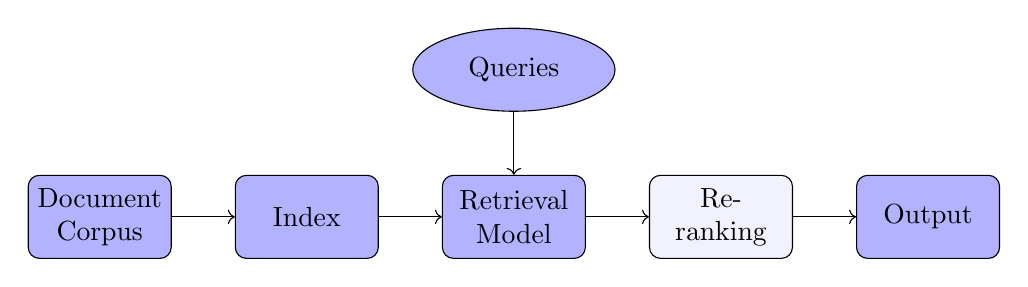
\begin{tikzpicture}[node distance=0.8cm, auto]

% Styles for boxes
\tikzstyle{box} = [rectangle, draw, fill=blue!10, text width=4.5em, text centered, rounded corners, minimum height=3em]
\tikzstyle{user} = [ellipse, draw, fill=blue!30, text width=4.5em, text centered, rounded corners, minimum height=3em]

% Nodes
\node [box, fill=blue!30] (corpus) {Document Corpus};
\node [box, fill=blue!30, right=of corpus] (index) {Index};
\node [box, fill=blue!30, right=of index] (model) {Retrieval Model};
\node [user, above=of model] (query) {Queries};
\node [box, fill=blue!5, right=of model] (rerank) {Re-ranking};
\node [box, fill=blue!30, right=of rerank] (output) {Output};

% Edges
\draw[->] (corpus) -- (index);
\draw[->] (query) -- (model);
\draw[->] (index) -- (model);
\draw[->] (model) -- (rerank);
\draw[->] (rerank) -- (output);

\end{tikzpicture}
\caption{Depiction of a basic retrieval pipeline, with optional re-ranking step. The process begins with a document corpus, which is indexed to facilitate efficient retrieval. Given the information need of a user in the form of a query, the retrieval model returns the most relevant documents. Optionally, the documents can be re-ranked using a re-ranking model which is usually more resource intensive.}
\label{fig:reranking_pipeline}
\end{figure}

\subsection{Baseline Retrieval Models}\label{sec:baseline-retrieval-models}
First, we will look at the basic retrieval models, which are used as baselines in this thesis.
They have been chosen, because they were shown to be effective on the used dataset in previous work~(\cite{goeuriot:2021}).
Both models use the implementation in the Terrier IR platform~(\cite{ounis:2005}).

\subsubsection{TF-IDF}\label{sec:tf-idf}
Term Frequency-Inverse Document Frequency (TF-IDF) is one of the most prevalent weighting schemes in information retrieval.
It aims to measure the importance of a term in a document relative to a collection of documents or corpus.
The central intuition is that terms that appear frequently in a document but not in many other documents in the corpus are significant and thus should be given higher weight.
\\\\
Given a term \( t \) and a document \( d \) in a corpus \( D \):
\[ \text{TF-IDF}(t, d, D) = \text{TF}(t, d) \times \text{IDF}(t, D) \]
Where \( \text{TF}(t, d) \) is the term frequency of term \( t \) in document \( d \) and 
\[ \text{IDF}(t, D) = \log \left( \frac{|D|}{1 + \text{df}(t, D)} \right) \]
with \( |D| \) being the total number of documents in the corpus and \( \text{df}(t, D) \) is the number of documents containing term \( t \).
\\
In the Terrier IR platform, the implementation of TF-IDF uses variants of the TF and IDF components.
For Term Frequency, the Robertson's TF formulation~(\cite{robertson:2004}) is used, which incorporates an additional parameter, that adds a saturation effect to the term frequency.
For IDF, the original formulation by Sparck Jones~(\cite{sparck:1972}) is applied.

\subsubsection{DPH}\label{sec:dph}
Divergence from Randomness (DFR) is a framework in information retrieval that assigns term weights based on the divergence of the actual within-document term frequency distribution from a random term frequency distribution~(\cite{amati:2006}).
The DPH (Divergence from randomness using the Hyper-geometric distribution model) is one of the models derived from the DFR framework.
\\
The principle behind DFR is that terms that are informative in a document will have a distribution that deviates significantly from what would be expected if terms were distributed randomly.
While TF-IDF emphasizes the importance of terms based on their frequency in a document and their inverse frequency in the corpus, DPH focuses on the divergence of a term's distribution from what would be expected under a random distribution.
Specifically, DPH assesses the divergence using the hyper-geometric distribution.
In essence, where TF-IDF weights terms based on their prominence and rarity, DPH weights them based on how much their occurrence pattern deviates from randomness.
The implementation in the Terrier IR platform follows the original formulation by \cite{amati:2006}.


\subsection{Transformer-based Retrieval Models}\label{sec:transformer-retrieval-models}
As mentioned in earlier sections, transformer-based models have been shown to be effective on a variety of tasks, including information retrieval.
There are different approaches of how transformers can be used for retrieval, a brief overview of methods used in this thesis is given here.
\\\\
Two of the most common transformer based architectures are cross-encoder and bi-encoder models.


\subsubsection{Cross-Encoders vs. Bi-Encoders}\label{sec:cross-encoders}
\begin{table}[h]
    \centering
    
    \begin{tabularx}{\textwidth}{l>{\centering\arraybackslash}X>{\centering\arraybackslash}X} % Center-align X columns
        \toprule
        \textbf{Aspect} & \textbf{Bi-Encoder} & \textbf{Cross-Encoder} \\
        \midrule
        Input & Separate embeddings & Combined input \\
        \addlinespace
        Embedding computation & Independent & Joint \\
        \addlinespace
        Output & Dense vector & Scalar score \\
        \addlinespace
        Retrieval stage & First-stage & Re-ranking \\
        \addlinespace
        Efficiency & High & Lower \\
        \addlinespace
        Interaction modeling & Limited & High \\
        \addlinespace
        Use-case & Large-scale & Re-ranking \\
        \bottomrule
    \end{tabularx}
    \caption{Comparison between Bi-Encoder and Cross-Encoder in the context of information retrieval.}
    \label{tab:encoder_comparison}
\end{table}

Bi-Encoders independently embed queries and documents using transformer models like BERT~(\cite{devlin:2018}) or T5~(\cite{roberts:2019}).
For the document collection, this can be done offline, since the embeddings are independent of the query.
This separation allows them to efficiently process large datasets since the embeddings can be pre-computed and stored.
It also enables rapid relatively quick retrieval, since only the embedding for the current query has to be calculated on the spot.
The following retrieval step is then done by computing the similarity between the query and each document in the collection, which is a relatively fast operation.
\\
Cross-Encoders, on the other hand, take a combined input sequence of both query and document and produce a scalar relevance score.
This joint modeling enables them to capture the interaction and nuances between a query and a document.
Due to their fine-grained interaction modeling, Cross-Encoders outperform Bi-Encoders in terms of precision in retrieving relevant documents.
However, the need to process each query-document pair individually makes them computationally demanding, especially for large datasets.
As a result, they are typically only used in second-stage retrieval, where the objective is to re-rank the top results obtained from an initial retrieval method.
\\
The following sections describe the different transformer-based retrieval models used in this thesis.
\subsubsection{MonoT5 + DuoT5}\label{sec:monot5-duot5}
MonoT5 and DuoT5~(\cite{roberts:2019}), are based on previous work by \cite{nogueira:2019}, who introduced monoBERT and duoBERT, first applying transformer architecture to the task of document ranking.
The general idea is to first use a baseline retrieval model like BM25 to retrieve an initial set of relevant documents.
Then, the query and each document in the initial set are concatenated and fed into the mono version of the transformer model, which produces a scalar score for each query-document pair.
The documents with the highest scores get then fed into the duo model, which takes the query and each possible pair of documents as input, outputting a probability of one document being more relevant than the other.
Given those scores, the documents are re-ranked another time, serving as the final output of the retrieval pipeline.
The main difference between the BERT and T5 versions, is that for BERT the [CLS] token from embedding the query and the document can be used as input to a single layer neural network, to output a probability of the document being relevant.
Since there is no [CLS] token for models in the T5 family, as they are sequence-to-sequence model, this part is done using an input template:
\begin{equation}
    \text{Query: \emph{q} Document: \emph{d} Relevant:}
\end{equation} 
where the model is fine-tuned to produce the token \emph{true} or \emph{false} given query \emph{q} and document \emph{d}.
\\
At inference, softmax is applied to the \emph{true} and \emph{false} tokens only, the scores are then calculated using the probability of the \emph{true} token.
This works analogously for the Duo version of both models, by just adding the second document.
MonoT5 and DuoT5 both belong to the family of cross-encoder models, as described in Section~\ref{sec:cross-encoders}, sharing the general characteristics of those models.
\\
This model architecture allows for accurately tuning performance vs. accuracy, by parameterizing how many documents are filtered in each step, making the model suitable for different usecases.
\\
In this thesis, the retrieval dataset is small, so the first retrieval step using BM25 is omitted, directly feeding all documents to the monoT5 model.

\subsubsection{ColBERT}\label{sec:colbert}
ColBERT~(\cite{khattab:2020}) is another BERT based model for document ranking.
It shares similarities with the general Bi-Encoder architecture, but introduces some modifications to improve performance.
Instead of representing each document and query as a single vector, ColBERT uses a set of vectors to represent contextualized embeddings for each token in the document or query.
For the documents, this can again be done offline, so that at the retrieval stage, only the embeddings for the query have to be generated and compared to the documents.
The relevance score for document $d$ given query $q$ is estimated using their late interaction model, in which maximum cosine similarity between all query term embeddings and document term embeddings is calculated, and then summed over for all query terms.
This allows for a more fine-grained mapping between query and document terms, also allowing for more fine-grained meaning of different terms.
An efficient computation of the similarity calculation allows ColBERT to scale much better, compared to feeding BERT the query and each document as input.
\\
The ColBERT architecture can generally be used for re-ranking or for end-to-end retrieval.
In the second case, an additional step is added in which the complete collection is filtered for relevant documents using similarity search for finding documents that contain similar terms as the query.
Then in the second step, the remaining documents are re-ranked using the maximum similarity metrics.
\\
Since the dataset used in this thesis is relatively small, we can directly use the re-ranking approach on all documents.


\subsection{Evaluation of Retrieval Models}\label{sec:evaluation-of-retrieval-models}
Evaluation metrics are important for the automatic assessment of retrieval model performance.
They provide a quantitative measure of how well a system retrieves relevant documents in response to a user's query.
Compared to other tasks like classification or regression, the evaluation of retrieval models is more challenging, since the evaluation metrics are not as intuitive.
Instead of a single correct answer, there are multiple documents that could be considered relevant to a query, which can be retrieved in different permutatons.
To be able to judge different retrieval methods, true relevance values for document-query pairs have to be defined by human assessors.
\\
There are multiple metrics which are widely used in information retrieval tasks:
\begin{itemize}
    \item \textbf{Precision}: Measures the fraction of retrieved documents that are relevant.
    \item \textbf{Recall}: Captures the fraction of relevant documents that are retrieved.
    \item \textbf{F1 Score}: The harmonic mean of precision and recall.
    \item \textbf{Mean Average Precision (MAP)}: The average precision scores for each query, considering the ranking order.
    \item \textbf{Mean Reciprocal Rank (MRR)}: The average of the reciprocal ranks of the first relevant document for each query.
    \item \textbf{Normalized Discounted Cumulative Gain (nDCG)}: Considers both the ranking and the relevance grade of retrieved documents.
\end{itemize}
Given the context of our dataset, which contains multiple queries with documents ranked for relevance between 0 and 3, and has relevance ratings for each document in the dataset, the nDCG metric is the most suitable one.
Specifically, nDCG@10 is used, setting a cutoff value after which additionally retrieved documents are not evaluated anymore.
The formula for nDCG@k is as follows:
\[ \text{nDCG@k} = \frac{\text{DCG@k}}{\text{Ideal DCG@k}} \]
where DCG@10 is the discounted cumulative gain at position 10, and Ideal DCG@10 is the DCG@10 score for the ideal ranking.
DCG@k is defined as:
\[ \text{DCG@k} = \sum_{i=1}^{k} \frac{2^{r(d_i,q)} - 1}{\log_2(i + 1)} \]
where $r(d_i,q)$ is the relevance rating of document $d_i$ for query $q$.
The ideal ranking is the ranking of documents for a query, which maximizes the DCG@10 score.
\\


\subsection{Evaluation of machine translation systems using Retrieval Models}\label{sec:eval-mts-ir}
In the field of evaluating NLP tasks, information retrieval techniques have been mainly used to evaluate machine translation systems.
Since both question answering and machine translation are sequence-to-sequence tasks with multiple correct answers, there are similarities in the evaluation process.
\\
For machine translation, a model is given a source sentence, and has to produce a target sentence in another language.
Those systems are usually evaluated given a ground truth reference sentence, which is compared to the predicted sentence.
Traditionally, methods like BLEU~(\cite{papineni:2002}), ROUGE~(\cite{lin:2004}) or METEOR~(\cite{banerjee:2005}) are used to compare the predicted sentence to one or multiple reference sentences.
There are multiple versions of those metrics with slightly different parameters, which mostly differ in what sequences of tokens are compared (1-gram, 2-gram, 3-gram, 4-gram, longest common sub-sequence), how precision and recall are weighted and how the results are smoothed.
In the end, all of those metrics generate a similarity score between the predicted and the reference sentence, which can be used to compare different models.
\\
Alternative approaches incorporating ranking methods have been proposed as well.
\cite{duh:2008} argue, that the final goal is to compare different ML systems, so why first predict the quality of the systems individually, when they could be compared directly.
He shows that ranking methods like RankSVM~(\cite{joachims:2002}) and RankBoost~(\cite{freund:2003}) can be applied to rank different candidate translations against the reference, while generating similar scores to BLEU on the same feature set.
When incorporating intra-set features, the ranking methods outperform BLEU and smoothed BLEU.
\\
Another approach, this time based on learning-to-rank methods, is proposed by \cite{li:2013}.
Again, they compare multiple translation candidates to a reference sentence, but here they use listwise learning-to-rank methods to generate a ranking of the candidates.
The objective of listwise ranking is to train a ranking function, which minimizes the loss between the predicted ranking and the ground truth human generated ranking on a training set.
The trained model is then evaluated on a test set.
Similar to \cite{duh:2008}, they show that the ranking based methods can outperform other automatic metrics in terms of correlation with human judgement.
\\
\cite{guzman:2019} use neural methods to incorporate syntactic and semantic information into the evaluation process.
They train a pairwise ranking model, which compares to candidate sentences given the reference and returns which one is the better translation.
Even tough they do not outperform other state of the art methods, they deliver competitive results while staying closer to the human evaluation framework.
\\
\\
This overview shows, that information retrieval methods have successfully been applied to the task of evaluating machine translation systems.
But those approaches are hard to transfer to the task of evaluating question answering systems, since the evaluation metrics are not directly applicable.
All machine translation evaluation methods mentioned here, compare the set of candidate translations to a single reference translation.
This is not applicable to long form question answering.
Here, multiple different answers can be correct, but still very different from each other.
So, even though information retrieval methods are applied here as well, the evaluation approach is fundamentally different.
\\
In this thesis, retrieval methods are used to rank generated answers for a given question against a set of rated reference answers which can differ from each other drastically.

\section{Summary}
In this chapter, we present an overview of the current state of research in the field of evaluating large language models for question answering.
Additionally, concepts of information retrieval that are relevant for this thesis are introduced.
\\
Section~\ref{sec:long-form-qa-difficulties} shows, that the evaluation of long form question answering is challenging, since the answers are free form text, and not only a single entity, number or multiple choice option.
This leads us to the investigation of how retrieval methods can be used to evaluate long form question answering.
Since retrieval methods have already been used to evaluate machine translation systems, we give an overview of those methods in Section~\ref{sec:eval-mts-ir}.
Even tough some similarities exist between the two tasks, the evaluation methods are not directly transferable.
\\
For this reason, we formulate the evaluation tasks differently.
Instead of ranking multiple candidates against one reference text, we rank one candidate against multiple reference texts.
\\
In the following Section, we introduce the Experimental Setup, including the dataset collection, ranking pipeline construction and the generation of LLM answers.
\chapter{Experimental Setup}\label{experimental-setup}
This chapter describes the experimental setup of this thesis, starting with the data collection and preparation process as well as an analysis of the resulting dataset.
Afterward, we describe the retrieval pipeline development and how the pipelines are evaluated.
Finally, the generation of LLM answers to the different queries is presented.

\section{Overview}\label{sec:overview}
The final goal of this project is to have a pipeline with which the answers of different LLMs can be ranked, in comparison to human answers.
To construct a pipeline like this we first need a dataset consisting of questions as well as human answers to these questions.
Those human-generated answers need to be ranked according to how well they answer the given question.
Subsequently, a retrieval pipeline is developed, which can rank the answer to a given question following the ranking of the human answers.
Finally, the answers generated by different LLMs can be ranked using the developed retrieval pipeline.
Assuming the effectiveness of the retrieval pipeline in ranking the answers according to human expectations, we expect that the ranking of LLM-generated answers will closely align with the rankings a human evaluator would assign.
A ranking of multiple LLM answers in this fashion allows us to compare long-form question-answering capabilities between different LLMs or between different prompting strategies for the same LLM, by comparing the ranking positions of the generated answers.

Since a dataset for this task has not been collected before, we first need to adapt an existing dataset for our use case.
Then, different retrieval methods are compared on the dataset, to find the one that ranks the available human-generated answers most similarly to human annotators.
Finally, the LLMs have to be selected for evaluation, and the answers generated by them have to be ranked using the most effective retrieval method.

\section{Data Collection and Preparation}\label{sec:dataset}
The dataset is based on the test set of the CLEF eHealth 2021 dataset \cite{goeuriot:2021:Consumer}.
It was originally intended to evaluate the ability of retrieval systems to provide credible, readable, and relevant answers to laypersons' health questions.

\subsection{CLEF eHealth 2021 Dataset}
The test set consists of 55 health-related queries which either stem from Reddit or Google search trends.
While the Reddit-sourced queries are well-formulated questions about specific health topics, the queries from Google search trends are not necessarily phrased as questions but rather as classical keyword-based search queries.

In addition to the queries, the dataset includes a collection of web documents and social media content.
The web documents were mainly obtained from the CommonCrawl archive, containing a diverse range of 600 domains.
This list of domains was created by the authors by executing medical queries via Microsoft Bing API and was augmented by adding known reliable and unreliable health-related websites.
The dataset was expanded by incorporating social media comments and posts from Reddit and Twitter.
The comments and post were collected by posting manually generated search queries based on 150 pre-selected health topics and retrieving relevant responses.

To get evaluations in each of the three categories (relevance, readability, and credibility), each query was assigned 250 documents based on rank-biased precision (RBP)-based Method A~(\cite{moffat:2008:Rank}).
RBPA is a method for choosing which documents from a pool of documents to select for evaluation by human annotators.
The pool of documents in this case is the collection of web documents and social media content returned by the participating teams of the shared task, as well as the organizer's baseline systems.
From this, documents are evaluated based on their rank in different runs and then scored according to the three different metrics.
A more detailed description of the pooling method can be found in \cite{lipani:2017:Fixed}.

After the 250 documents per query are selected, the documents are evaluated by humans for credibility, readability, and relevance.
In total, there are 26 annotators, each annotating documents for between 1 and 4 queries completely.
The annotators were not medical experts but received written training material.
In the end, three annotations were made for a total of $11 357$ unique documents.
This differs from the total amount of annotations in each metric which is $12 500$, since some documents were annotated multiple times but for different queries.

The annotations for relevance and readability are in the categories 0 (not relevant / not readable), 1 (somewhat relevant / somewhat readable), and 2 (highly relevant / highly readable).
For scoring credibility, a category 3 exists, which is also interpreted as highly credible.
The reasoning for this additional ranking score for credibility is not given in the original paper.

The following sections describe how the dataset was collected and prepared for the experiments in this thesis.
\subsection{Dataset Collection}
There are two ways of accessing the CLEF eHealth 2021 dataset.

Option one is to download the indexed collection directly.
This index does not contain the full text of the documents, so it can not be used to compare the original documents against newly generated answers.

The second option is to download all documents individually, given their IDs.
In theory, this can be achieved by using the provided scripts in the organizer's GitHub repository\footnote{\url{https://github.com/CLEFeHealth/CHS-2021}}.
Scripts are provided to download the documents from the CommonCrawl archive, as well as the social media content directly over the respective APIs.

Unfortunately, with Twitter shutting down their free tier of the API, at the beginning of April 2023, this is now only possible with a prohibitively expensive paid tier.

For Reddit, those API changes followed just a few months later, making it impossible to download social media content from Reddit as well.
Even though we started downloading some Reddit content before those changes, the already slow access to the Reddit data did not allow for downloading all the content in time.

This was unfortunate timing, but since the organizers of the CLEF eHealth task reported in their paper that the human credibility assessments of social media documents were significantly lower than those of web documents, we decided to only use the web documents for our dataset.
The web documents are easily accessible via the CommonCrawl archive.


Before accessing all relevant documents from the CommonCrawl archives, the list of documents is filtered to only include documents that are annotated for at least one query.
Discarding all documents from Reddit and Twitter, as well as web documents that are not assessed for any query, results in a total of $6692$ documents downloaded from the CommonCrawl archive using a slightly modified version of the provided script.
This provides us with WARC files for the relevant documents.

Since all social media content is discarded, the number of queries for which documents are available is reduced to 50, since of the total 55 queries, 5 queries only have social media content associated with them.

\subsection{Preprocessing}
The files in the WARC format contain the full HTML of the web documents.
Before being able to compare the content to the generated answers, the HTML is extracted from the documents.
HTML elements containing fewer than 50 characters in the element body are discarded, assuming they are not relevant to the content of the document (e.g. fields of navigation bars).
Then, the plain text is extracted using the ChatNoir Resiliparse Library\footnote{\url{https://resiliparse.chatnoir.eu/en/stable/}}.

The final dataset now consists of 50 queries, each of which has between 39 and 249 documents associated with it that are evaluated for relevance, readability, and credibility.

\section{Analysis of the Final Dataset}
We now go more in-depth on the properties of the final dataset, considering the type of queries, the number of answers per query, and the length of the answers.

The total number of queries in the final dataset is 50, each of which is accompanied by between 39 and 249 answers.
The number of answers depends on how many of the given answers in the base dataset by \cite{goeuriot:2021:Consumer} were, still available, i.e. not from Reddit or Twitter.
Since this was not the same for all queries, the number of answers per query varies.
On average, there are about 178 evaluated documents per query available.

\subsection{Queries}
We identify two different query types in the dataset: questions and keyword queries.
Questions are queries that are formulated as a question, e.g. ``Is a ketogenic diet suitable for people with diabetes?'', while keyword-based queries are more in the style of search engine queries, e.g. ``keto diet diabetes''.
\begin{table}[tb]
\centering
\begin{tabularx}{\textwidth}{XX}
\hline
\textbf{Keyword-Based Queries} & \textbf{Question-Type Queries} \\
\hline
best apps daily activity exercise diabetes & What are the most common chronic diseases? \\
\hline
my risk for developing type 2 diabetes & Is a ketogenic/keto diet suitable for people with diabetes? \\
\hline
multiple sclerosis stages phases & Can diabetes be cured? \\
\hline
\end{tabularx}
\caption{Samples of Keyword vs Question Type Queries}
\label{table:querie-samples}
\end{table}
Table \ref{table:querie-samples} shows some examples of the two query types.
Query topics are diverse, ranging from general queries about chronic diseases to specific questions about the suitability of certain diets for people with diabetes.

\begin{figure}
\centering
\includegraphics[width=\textwidth]{images/num_words_per_query.pdf}
\caption{Boxplot of the number of words per query, split by query type. Keyword queries are shorter than question queries with a median of 4 words compared to 7 words for the question queries.}
\label{fig:num_words_per_query}
\end{figure}
In total, we identify 17 question-style queries and 33 keyword-style queries.
Figure \ref{fig:num_words_per_query} shows the number of words per query for both query types.
As expected, the keyword queries are shorter than the question queries, with a median of 4 words compared to 7 words for the question queries.
The shortest query is only two words long, while the longest query is 20 words long.
In a later section, we investigate the differences in answer ranking of the different models depending on the two query types.
\subsection{Documents}
\begin{table}[tb]
\centering
\begin{tabular}{ll}
\hline
\textbf{Domain} & \textbf{Occurrences} \\
\hline
www.healthline.com & 603 \\
www.nationalmssociety.org & 419 \\
www.ms.org.au & 198 \\
jhu.pure.elsevier.com & 191 \\
www.msif.org & 183 \\
www.psychologytoday.com & 161 \\
www.urotoday.com & 155 \\
www.news-medical.net & 150 \\
www.sleepfoundation.org & 141 \\
www.aafp.org & 139 \\
\hline
\end{tabular}
\caption{Top 10 Most Frequently Occurring Domains}
\label{tab:top_domains}
\end{table}
The documents in the dataset are scraped from a total of 234 different domains.
Table \ref{tab:top_domains} shows the top 10 most frequently occurring domains in the dataset.
Most domains are health-related, belonging to either health organizations, medical journals, or health news websites.
Some domains are more general, e.g. there are also wikipedia.org pages in the dataset, as well as some domains from essay writing or homework help websites.
A total of 133 domains show up less than 10 times in the dataset, while 44 domains show up only once.

\begin{figure}[tb]
\centering
\includegraphics[width=\textwidth]{images/num_words_per_passage.pdf}
\caption{Histogram of the number of words per document. The plot is cut at 15,000 words, which excludes 120 or 2\% of the documents. The median number of words per document is 1354, while the mean is 2901.}
\label{fig:num_words_per_document}
\end{figure}
After preprocessing, the documents are cleaned of all HTML tags and HTML elements containing fewer than 50 characters.
Figure \ref{fig:num_words_per_document} shows that the number of words per document is very high, with a median of 1354 words and a mean of 2901 words.
This is natural for documents scraped from the web, which not only contain the main text but also navigation bars, footers, sidebars, and other elements.
Those can not be fully removed with our trivial preprocessing methods.
\subsection{Document Ratings}
The document metrics in the dimensions of readability, credibility, and relevance are the human annotations from \cite{goeuriot:2021:Consumer}.
Documents can have multiple ratings for each dimension if they are annotated for multiple queries.
This means that the total number of ratings per dimension (8902) is higher than the number of documents in the dataset (6692).


In general, a surprisingly high number of documents are rated as not relevant to the given query.
Figure \ref{fig:heatmap_rel_cred_read} shows three heatmaps, with each relevance category being displayed in a separate heatmap.
Documents rated with 0 relevance make up nearly half of the dataset and generally have lower credibility and readability scores.
The most relevant documents are generally also the most credible and readable ones.
The correlation between relevance and credibility is only 0.08, so while it is slightly positive, it is not very strong.
For readability and relevance, the correlation is 0.22, which is slightly stronger, but still does not show a strong connection.
This can be interpreted as the relevance of a document being independent of its credibility and readability, which shows that the annotators were able to judge the relevance of a document independently of its credibility and readability.
\begin{figure}
\centering
\includegraphics[width=\textwidth]{images/heatmap_qrels.pdf}
\caption{Three heatmaps, one for each relevance category, plotting credibility against readability.
The total number of documents with the given relevance ranking is in the title of the heatmap.
In all three heatmaps, the highest number of documents is concentrated in the range between 1 and 2 for both credibility and readability, with 2 credibility and 2 readability being the most common combination.
}
\label{fig:heatmap_rel_cred_read}
\end{figure}

\subsection{Documents with Ratings for Multiple Queries}\label{sec:documents-with-multiple-ratings}
As mentioned previously, some documents have multiple ratings for different queries.
In total 875 documents are rated for multiple queries, with the highest number of individual annotations for a single document being 18.
Documents with multiple ratings are often general articles about a certain topic, e.g. ``What is Multiple Sclerosis?''.
Those are then retrieved for multiple queries that focus on different aspects of the topic, e.g. ``List of multiple sclerosis symptoms'' and ``Can I pass multiple sclerosis to other family members?''.
As expected, the different relevance ratings for the same document are often different, since the relevance of a document depends on the query.
Interestingly, we also find that the credibility and readability ratings for the same document can be different.
In Appendix \ref{appendix:dataset}, we show an example of a document with multiple ratings for different queries.
The 15 different ratings cover nearly all possible combinations of relevance, credibility, and readability.

As all documents for one query are annotated by the same person according to \cite{goeuriot:2021:Consumer}, we assume that the annotators were consistent in their ratings for the same query.
Because we are only interested in the ranking of the documents for one query at a time, we do not remove or aggregate the scores, as this could alter the ranking of the documents compared to documents that were only ranked for this specific query.

\section{Retrieval Pipeline Development}
In this section, the implementation of the different retrieval pipelines is discussed.
The baseline models (DPH and TF-IDF), as well as the ColBERT version 1 and the monoT5/duoT5-based pipelines, are implemented in the PyTerrier framework by \cite{pyterrier:2020:Declarative}, which is a Python API for the Terrier IR Platform~(\cite{macdonald:2012:From}).
The ColBERT version 2 pipeline is based on the original implementation provided by the authors\footnote{\url{https://github.com/stanford-futuredata/ColBERT}}.

Those pipelines are all designed to retrieve the most relevant documents for a given query.
Since our dataset also contains annotations for readability and credibility, we also want to be able to retrieve documents based on those criteria.
To extend the retrieval pipelines for those metrics, we experiment with adding external scores to the retrieval process.
This is described in section \ref{sec:external-scores}.

\subsection{Retrieval Setup}
The retrieval setup in this work differs from the usual retrieval setup, in which a large document collection is indexed, and then multiple queries are run against the index using different retrieval models.
In our case, we build separate indices for each query, containing only the documents that are evaluated for that query.
This ensures that each document that is retrieved for a query is also evaluated for that query.

\subsection{Baseline Models}
This section describes the implementation of the baseline models, namely DPH and TF-IDF.
For both models, the basic indexing function of PyTerrier is used, which indexes and preprocesses the documents.
Preprocessing is done with the default values, which include the following operations:
\begin{itemize}
    \item{\textbf{Tokenization}, for splitting the text into individual words or tokens. The default PyTerrier tokenizer splits text on non-alphanumeric characters. Additional rules to discard tokens that are longer than 20 characters, contain more than 4 digits or contain the same character more than 3 times in a row are applied. All tokens are also converted to lowercase.}
    \item \textbf{Stopword removal}, to remove tokens that do not contain information about the content. We use the default PyTerrier stopword list.
    \item \textbf{Stemming}, to remove the different endings a token can have, leaving only the root of the word. The Porter stemmer, a rule-based stemmer, is used here.
\end{itemize}
The resulting inverted index contains all remaining tokens and a mapping from each token to the documents in which it occurs.

The two retrieval models TF-IDF and DPH are then applied using the default parameters.
More details about the models can be found in section \ref{sec:baseline-retrieval-models}.


Both models are tested with and without query expansion.
We use BO1 query expansion, which is a query expansion method that uses the documents retrieved by the original query to expand the query.
It adds terms from the retrieved documents to the original query based on informativeness, which is a measure of how frequently the term occurs in the documents compared to how frequently it occurs in the whole collection.
Terms that occur more frequently in the retrieved documents than in the collection are added to the query.
Afterward, the expanded query is run against the index again, and the documents are ranked according to the new query.


\begin{figure}[tb]
    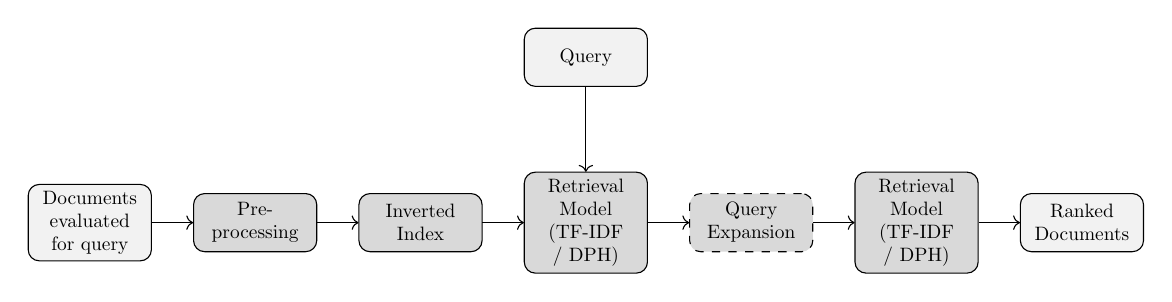
\begin{tikzpicture}[node distance=3cm, every node/.style={scale=0.7}]
    \tikzstyle{box} = [rectangle, draw, fill=gray!10,  text width=2cm, text centered, rounded corners, minimum height=3em]
    \tikzstyle{process} = [rectangle, draw, fill=gray!30,  text width=2cm, text centered, rounded corners, minimum height=3em]
    \node (docCol) [box] {Documents evaluated for query};
    \node (preprocess) [process, right of=docCol] {Pre-\\processing};
    \node (invertedindex) [process, right of=preprocess] {Inverted Index};
    \node (retrieval) [process, right of=invertedindex] {Retrieval Model (TF-IDF / DPH)};
    % query expansion with dotted line around
    \node (qe) [process, right of=retrieval, dashed] {Query Expansion};
    \node (reranking) [process, right of=qe] {Retrieval Model (TF-IDF / DPH)};
    \node (ranked) [box, right of=reranking] {Ranked Documents};
    \node (query) [box, above of=retrieval] {Query};

    \draw [->] (docCol) -- (preprocess);
    \draw [->] (preprocess) -- (invertedindex);
    \draw [->] (invertedindex) -- (retrieval);
    \draw [->] (retrieval) -- (qe);
    \draw [->] (qe) -- (reranking);
    \draw [->] (reranking) -- (ranked);
    \draw [->] (query) -- (retrieval);

    \end{tikzpicture}
\caption{Baseline retrieval pipeline, using either TF-IDF or DPH as retrieval model with optional query expansion. This retrieves and ranks evaluated documents for a given query.}
\label{fig:baseline-pipeline}
\end{figure}
The resulting pipeline is shown in Figure \ref{fig:baseline-pipeline}.
This produces a ranked list of documents for each query, which can then be compared to the order of documents according to the human annotations.

\subsection{Transformer Models}
In addition to the baseline models, we also implement the transformer-based models ColBERT version 1 and 2, as well as the monoT5 and duoT5-based models.
The implementation of ColBERT version 1 and the monoT5/duoT5-based models is done in PyTerrier, while the implementation of ColBERT version 2 is done in the original implementation provided by the authors.

All mentioned models are based on a pre-trained model, which is at some point used to encode the query and the documents in different ways.
Both ColBERT versions are based on the BERT-base model, while the monoT5 and duoT5-based models are based on the T5 model.
The retrieval models themselves are fine-tuned on the MS MARCO passage ranking dataset~(\cite{bajaj:2016:MSMARCO}), a large-scale dataset for passage retrieval.

Transformer-based retrieval models usually require a first retrieval step using a less computationally expensive model like tf-idf, to reduce the number of documents that are fed to the transformer model.
Because in this thesis the retrieval dataset is small, the first retrieval step is omitted for all transformer-based models.

\subsubsection{ColBERT Version 1}
Using the ColBERT implementation for PyTerrier\footnote{\url{https://github.com/terrierteam/pyterrier_colbert}}, an end-to-end pipeline can be constructed from a pre-trained ColBERT model and a document collection.
In our testing, we use the pre-trained ColBERT checkpoint provided by the authors.

The checkpoint can directly be loaded in the PyTerrier framework, and then used to retrieve documents from the collection.
All settings are left at their default values.

\subsubsection{monoT5 and duoT5}
Like the ColBERT implementation, the monoT5 and duoT5 implementations are also available in PyTerrier\footnote{\url{https://github.com/terrierteam/pyterrier_t5}}.
Pre-trained checkpoints based on the MS MARCO dataset are provided by the authors.

The monoT5 pipeline uses the pre-trained checkpoint to encode each query with each of the associated documents.
From this encoding, a score is calculated for each query-document pair, and the documents are ranked according to this score.

The duoT5 pipeline is based on the monoT5 pipeline but uses the duoT5 re-ranker to re-rank the top 10 documents retrieved by the monoT5 pipeline.
Here, the pre-trained duoT5 checkpoint is used to encode the query and each possible pair of the top 10 documents, to determine which of the two documents is more relevant to the query.
Based on this order, the documents are re-ranked.

Again, all parameters are left at their default values.

\subsubsection{ColBERT Version 2}
Unlike the other transformer-based models, ColBERT version 2 is not available directly in PyTerrier.
Instead, we use the implementation provided by the authors of the model\footnote{\url{https://github.com/stanford-futuredata/ColBERT/tree/main}}.

The implementation works with any pre-trained checkpoint for the ColBERT version 2 model, with the MS MARCO checkpoint being downloaded by default.

\subsection{External scores for Readability}\label{sec:external-scores}
To improve retrieval effectiveness for readability, we experiment with adding pre-computed external scores to the retrieval process.

To estimate the readability of the documents in the dataset, different scores are calculated for each document.

The first score is the Flesch Reading Ease (FRE) score devised by \cite{kincaid:1975:Derivation}, which is a score between 0 and 100, with higher scores indicating easier-to-read text.
It is calculated using the following formula, based on average sentence length (ASL) and average number of syllables per word (ASW):
\begin{equation}
    FRE = 206.835 - (1.015 \times ASL) - (84.6 \times ASW)
\end{equation}
We use the implementation provided by the textstat library\footnote{\url{https://pypi.org/project/textstat/}}.

This library also provides the second score, which is an aggregate of multiple similar scores, like the FOG score, the SMOG score, and the Coleman-Liau Index.
Those scores are all based on different text statistics, like the number of syllables per word, the number of words per sentence, or the number of characters per word.
More details about the different scores can be found in the documentation of the textstat library.

\section{Evaluation of Retrieval Pipelines}
In this section, we compare the effectiveness of the different retrieval pipelines.
We chose to evaluate the pipelines using nDCG@10, which was explained in section \ref{sec:evaluation-of-retrieval-models}.
nDCG is a suitable metric for our task, as it takes into account multiple different relevance/credibility/readability levels instead of only the binary relevant/not relevant distinction.
Furthermore, it emphasizes the importance of the top results, which we expect to be the most competitive ones against the LLM answers, so it is important to be able to distinguish between answers at the top level.
We chose a cutoff of 10 because even though the minimum available number of answers per query is 39, the number of relevant results is much lower.
\begin{table}[tb]
\centering
\begin{tabularx}{\textwidth}{lXXX}
\hline
Pipeline    & Relevance          & Readability        & Credibility        \\ \hline
DPH         & 0.643 & 0.742 & 0.539 \\
DPH\ (qe)     & 0.637 & 0.751 & 0.51  \\
TF-IDF     & 0.64  & 0.746 & 0.551 \\
TF-IDF (qe) & 0.636 & 0.751 & 0.557 \\
ColBERTv1      & 0.626 & 0.774 & 0.633 \\
ColBERTv2       & 0.634 & 0.799 & 0.65  \\
duoT5            & 0.64  & 0.805 & 0.714 \\
monoT5           & \textbf{0.645} & \textbf{0.813} & \textbf{0.722} \\
\hline
\end{tabularx}
\caption{Results of the transformer pipelines, shown as nDCG@10. The best results of the baseline pipelines are shown for comparison. All models are trained on the MS MARCO passage ranking dataset(\cite{bajaj:2016:MSMARCO}).}
\label{tab:transformer_pipelines}
\end{table}
\subsection{Baseline Pipelines}
Our baseline retrieval pipelines are the TF-IDF and BM25 pipelines, each once with and once without query expansion.
Effectiveness on all three metrics is similar for all pipelines, showing little difference between the strategies.
Table \ref{tab:transformer_pipelines} shows the retrieval performance of the baseline pipelines in the first four rows.
The rankings are closest to the human rankings for readability, scoring around 0.75 for all pipelines.
Relevance is lower than that, with scores around 0.64.
Since those models are designed to retrieve relevant documents, we would expect the relevance scores to be higher.
The credibility scores are the lowest, with scores around 0.55.

\subsection{Transformer Pipelines}
Table \ref{tab:transformer_pipelines} shows the nDCG@10 scores for the different transformer-based pipelines, compared to the best baseline results.
The monoT5 pipeline performs best on all three metrics, with scores of 0.645 for relevance, 0.813 for readability, and 0.722 for credibility.
Re-ranking the top 10 results using duoT5 made the results slightly worse in all metrics.
ColBERTv2 shows a slight improvement over ColBERTv1 but is still worse in relevance while being better in readability and credibility.

In general, the transformer-based models perform very similarly to the baseline models in terms of relevance, but all transformer-based models achieve higher scores on readability and credibility.

\subsection{External Document Scores}
Because we did not find any retrieval models that consider readability as the main ranking dimension, we investigate adding external scores to the ranking process.
First, the statistical scores described in Section \ref{sec:external-scores} are calculated for all documents in the dataset.
We then compare the calculated scores to the readability scores assigned by the human annotators.
For our dataset, we do not find a strong correlation between the human-annotated readability scores and the statistical scores.
The Flesch Reading Ease score has a correlation of 0.177 with the readability scores, while the full textstat score has a slightly negative correlation of -0.147.
Those correlations are not strong enough to justify using the statistical scores as a proxy for readability.

This might be connected to the fact that the documents in our dataset are scraped from the web, which means that even after preprocessing they still contain noise not accounted for by the statistical scores, which are intended for the use on clean text.

\section{Generating LLM Responses}
We now introduce the LLMs that selected for the experiments, and the steps taken to get the generated answers from the LLMs.
Additionally, the different prompting strategies that are used to generate the responses are described.

\subsection{Selection of Language Models}
We select multiple LLMs for our experiments, which differ in the number of parameters, amount and type of training data, and the type of pre-training and fine-tuning.

\subsubsection{GPT-2}
As a simple baseline and to investigate how an increased number of parameters affects the ranking results, we select different sizes of the GPT-2 model, namely the base, medium, large, and XL versions.
Those models only differ in the number of parameters, which are 124M, 355M, 774M, and 1.5B respectively, while the training objective and the training data are the same for all models.
The dataset used for pre-training is the WebText dataset, which contains 40 GB of web text, which is scraped from URLs shared on Reddit that received at least 3 upvotes.
Other than this pre-training, the models are not fine-tuned to any specific task.

\subsubsection{Models optimized for dialog}\label{sec:dialog-models}
Dialog-optimized models are fine-tuned for the task of interacting with a human in a dialog, usually as a chatbot.
This is currently the use case of LLMs that comes closest to the task of long-form question answering, so including models optimized for dialog is a natural choice.
To make a model suitable for directly interacting with humans, different fine-tuning objectives are used in which the behavior of the model is aligned with the expectations of the human.

The importance of this alignment is shown by \cite{ouyang:2022:Training}, who show that answers of their instruction-tuned model InstructGPT are preferred by humans compared to outputs by a model with over 100 times the number of parameters, but without any fine-tuning.

We select the following models:

The \textbf{Falcon} family of models, which was released in 2023 on HuggingFace\footnote{\url{https://huggingface.co/blog/falcon}}.
At the time of writing, there are three model sizes available, 7B, 40B, and 180B parameters, each as a foundation model or as an instruction-tuned model.
For our testing, we only use the small 7B instruction-tuned model.

According to the HuggingFace model card, the model is pre-trained on the RefinedWeb dataset by \cite{penedo:2023:The} and then fine-tuned on the GPTeacher\footnote{\url{https://github.com/teknium1/GPTeacher}}, GPT4All\footnote{\url{https://github.com/nomic-ai/gpt4all}} and Baize~(\cite{xu:2023:Baize}) datasets.
GPTeacher and GPT4All are both datasets of prompt-response pairs, while Baize is a dataset based on self-chats by ChatGPT, which have been seeded by questions from Quora, StackOverflow, and MedQuAD.

Unfortunately, the authors do not detail exactly how the data was used to fine-tune the model, as a scientific paper is still yet to be released.


\textbf{Llama 2}, a model introduced in 2023 by \cite{touvron:2023:Llama}.
It is available through the HuggingFace library, after agreeing to the terms of use posed by Meta.
It comes in three sizes, 7B, 13B, and 70B parameters.
For each of the sizes, the base language model, and a fine-tuned version for chat is available.
In our testing, we use the fine-tuned version in both the 7B and 13B sizes, since the 70B parameter model is too large to fit on the available hardware.

To create the chat model, the base model is first tuned using supervised fine-tuning, where the model is trained on a dataset of prompt-response pairs, which are all written by humans.

The next step is Reinforcement Learning with Human Feedback (RLHF), by which the model is aligned with human preferences. 
To generate a training set, humans are tasked to evaluate which of two generated responses to a given prompt they prefer.
Based on that data, a reward model is trained, which can then evaluate generated responses on a large scale.
The model is then fine-tuned to maximize the reward given by the reward model.

The RLHF training is done over multiple iterations, continuously improving the reward model and the chat model based on human feedback.
Additionally, they not only optimize for the helpfulness of the generated response but also evaluate for safety, instructing the model not to provide harmful content in that way.


\textbf{ChatGPT}, is the largest model we used, with 175B parameters. 
It was introduced by OpenAI at the end of 2022\footnote{\url{https://openai.com/blog/chatgpt/}}.
As a commercial product, it can only be accessed through the OpenAI API, which we did using the provided Python library.

With OpenAI becoming more secretive about their models since starting to monetize them, the exact training data and fine-tuning procedure are not known.
In their blog post, they state that the model is a close sibling to the InstructGPT model mentioned above.
This means the fine-tuning procedure is likely similar to the one described by \cite{ouyang:2022:Training} but with a larger model size.
The methods applied are similar to the ones used for the Llama 2 model, first using supervised fine-tuning, and then using RLHF to align the model with human preferences.


Table \ref{tab:language-models} gives an overview of all the used models, comparing parameter size pre-training and fine-tuning data, as well as fine-tuning methods.
In total, we use 8 different models, 4 of which are variants of GPT-2, while the others a different fine-tuned models for chat.
\begin{table}[tb]
\centering
\begin{tabularx}{\textwidth}{lllXXX}
\hline
\textbf{Model} & \textbf{Params} & \textbf{Release} & \textbf{Pre-training Data} & \textbf{Fine-tuneing Data} & \textbf{Fine-tuneing Methods} \\
\hline
GPT-2 Base    & 124M & \multirow{4}{*}{2019} & \multirow{4}{*}{WebText} & \multirow{4}{*}{-} & \multirow{4}{*}{-} \\
GPT-2 Medium  & 355M &                      &                          &  &  \\
GPT-2 Large   & 774M &                      &                          &  &  \\
GPT-2 XL      & 1.5B &                      &                          &  &  \\
\hline
Falcon 7B              & 7B      & 2023 & RefinedWeb           & GPTeacher, GPT4All, Baize & SFT \\
\hline
Llama 2 7B & 7B    & \multirow{2}{*}{2023} & \multirow{2}{*}{Proprietary} & \multirow{2}{*}{Proprietary} & \multirow{2}{*}{SFT, RLHF} \\
Llama 2 13B   & 13B   &  &                        &                         &  \\
\hline
ChatGPT                & 175B   & 2022 & Proprietary                & Proprietary & Proprietary \\
\hline
\end{tabularx}
\caption{Comparison of evaluated Language Models. SFT = Supervised Fine-Tuning, RLHF = Reinforcement Learning with Human Feedback}\label{tab:language-models}
\end{table}

\subsection{Prompting approaches}\label{sec:prompting-approaches}
How a LLM is prompted to complete a task has a large impact on the quality of the generated response.
\cite{reynolds:2021:Prompt} show this in the context of translating French to English.
They compare the effect of three different prompting strategies, finding that the most complex one leads to the best translations.
% They compare the effect of three different prompting strategies on the 6.7 B and 13 B parameter versions of GPT-3:
% \begin{enumerate}
%     \item \textbf{Strategy 1}\\Q: What is the English translation of \textit{french\_sentence} A: \textit{translation}
%     \item \textbf{Strategy 2}\\French: \textit{french\_sentence}\\English: \textit{translation}
%     \item \textbf{Strategy 3}\\A French phrase is provided: \textit{french\_sentence}\\
%     The masterful French translator flawlessly translates the phrase
% into English: \textit{translation}
% \end{enumerate}
% where \textit{french\_sentence} is replaced by the sentence to be translated before prompting the model, which then generates the \textit{translation}.
% According to their results in the BLEU metric, the first prompting strategy is outperformed by the other two.
% Of those two, the third one performs better on the smaller 6.7B model, while on the 13B model, they perform about equally well.
% Table \ref{tab:fr-en-prompting} shows the large differences in the BLEU score between the different prompting strategies.
% \begin{table}[tb]
% \centering
% \begin{tabularx}{\textwidth}{lXXX}
% \hline
% \textbf{Model} & \textbf{Strategy 1} & \textbf{Strategy 2} & \textbf{Strategy 3} \\
% \hline
% 6.7B & 15.9 & 23.5 & 26.5 \\
% 13B & 18.7 & 33.3 & 32.9 \\
% \hline
% \end{tabularx}
% \caption{BLEU scores for different prompting strategies for the 6.7B and 13B models of GPT-3, as reported by \cite{reynolds:2021:Prompt}}\label{tab:fr-en-prompting}
% \end{table}
Based on those results we use a similar approach of different prompting strategies for our experiments.
We use the following four strategies:
\begin{enumerate}
    \item \textbf{No Prompt:}\\ \textit{query}
    \item \textbf{QA Prompt:}\\ Q: \textit{query}\\A:
    \item \textbf{QuestionAnswer Prompt:}\\ Question: \textit{query}\\Answer:
    \item \textbf{MultiMedQA Promp:}\\ You are a helpful medical knowledge assistant. Provide useful, complete, and scientifically grounded answers to common consumer search queries about health.\\Question: \textit{query}\\Complete Answer:
\end{enumerate}
where \textit{query} is replaced by the query to be answered.
Based on the results of \cite{reynolds:2021:Prompt}, we expect the generated answers based on the MultiMedQA prompt to rank highest, followed by the QuestionAnswer prompt.
To restrict the influence of random variations in the generated responses, we generate 10 responses for each query and model.

\subsection{Generating Answers}
To generate answers for a given query, the query is passed to the LLM using one of the prompting strategies described above.
Most LLMs take additional parameters as input, which are used to guide the text generation process.
The following parameters are considered for the different models in our experiments:
\begin{itemize}
    \item \textbf{max new tokens}: This parameter defines the maximum number of new tokens to be generated by the LLM, limiting the length of the generated output.
    \item \textbf{temperature}: The temperature parameter controls the randomness in the generation process. A higher temperature value increases randomness in the output, while a lower value leads to more deterministic outputs.
    \item \textbf{top k}: This parameter sets a threshold for the number of most likely next tokens to consider at each step of generation, only allowing the model to choose from the top k tokens. A higher value for k will increase the diversity of the generated output, while a lower value will decrease diversity.
    \item \textbf{top p}:  Also called nucleus sampling, specifies a cumulative probability threshold. The model will only consider the smallest set of tokens whose cumulative probability does not exceed the threshold.
    \item \textbf{repetition penalty}: This parameter is used to discourage the model from repeating the same phrases. A repetition penalty greater than 1 will decrease the likelihood of tokens that have already appeared in the generated text, so the model produces more diverse and less repetitive content.
\end{itemize}
Not all parameters are available for all models and the optimal values for each parameter differ between models.
We chose to set the same values for all models, to make the comparison between the models more consistent.
We did not try to find the optimal values for each model but instead used values we found to work well with all models in manual testing.

The \textbf{maximum number of new tokens} is set to 512 because that's the maximum length of the input for the GPT-2 models.

\textbf{Temperature} is set to 0.75, restricting the variability of the generated output, while still allowing for some randomness.

\textbf{Top k} is set to 50, and \textbf{top p} is set to 0.95, which both restrict the number of tokens the model can choose from to more likely tokens.

Finally, we set a \textbf{repetition penalty} of 1.2, which is a relatively low value, but still helps to reduce repetition in the generated output, which we found to be a common problem, especially for the GPT-2 models, but also for the smaller instructing tuned models.
Any additional parameters that are available for a model are left at their default values.

The generating of the answers is done in two different ways.
For ChatGPT, we use the OpenAI API to generate the answers, specifically using the model version ``GPT-3.5-turbo-0613''.
Since they do not provide any parameters apart from temperature and number of tokens, we only set those to our chosen values.

For all other models, we use the HuggingFace library to generate the answers.
This allows us to set all parameters as described above.
Each model is prompted ten times with each of the prompting strategies, resulting in 40 generated answers per query for each model.
\chapter{Results}\label{chapter:results}
In this chapter, we present the results of our experiments.
Starting with an evaluation of the retrieval pipelines, we follow with showing the effectiveness of the different LLMs on the rank-based implicit evaluation method.
The results and visualizations needed to evaluate the research questions formulated in the Introduction are presented.

\section{Evaluation of Retrieval Pipelines}
In this section, we compare the effectiveness of the different retrieval pipelines.
We chose to evaluate the pipelines using nDCG@10.
nDCG is a suitable metric for our task, as it takes into account multiple different relevance/credibility/readability levels instead of only the binary relevant/non-relevant distinction.
Furthermore, it emphasizes the importance of the pipeline being able to distinguish between answers at the top level by giving more weight to the top results.
We chose a cutoff of 10 because even though the minimum available number of answers per query is 39, the number of relevant results is much lower.
This cutoff also normalizes the rank position between the different queries, as the number of assessed documents per query varies.
\begin{table}[tb]
\centering
\begin{tabularx}{\textwidth}{lXXX}
\hline
Pipeline    & Relevance          & Readability        & Credibility        \\ \hline
DPH         & 0.643 & 0.742 & 0.539 \\
DPH\ (qe)     & 0.637 & 0.751 & 0.51  \\
TF-IDF     & 0.64  & 0.746 & 0.551 \\
TF-IDF (qe) & 0.636 & 0.751 & 0.557 \\
ColBERTv1      & 0.626 & 0.774 & 0.633 \\
ColBERTv2       & 0.634 & 0.799 & 0.65  \\
duoT5            & 0.64  & 0.805 & 0.714 \\
monoT5           & \textbf{0.645} & \textbf{0.813} & \textbf{0.722} \\
\hline
\end{tabularx}
\caption{Results of the transformer pipelines, shown as nDCG@10. The best results of the baseline pipelines are shown for comparison. All models are trained on the MS MARCO passage ranking dataset (\cite{bajaj:2016:MSMARCO}).}
\label{tab:transformer_pipelines}
\end{table}
\subsection{Baseline Pipelines}
Our baseline retrieval pipelines are the TF-IDF and BM25 pipelines, each evaluated once with and once without query expansion.
Effectiveness on all three dimensions is similar for all pipelines, showing little difference between the strategies.
Table \ref{tab:transformer_pipelines} shows the retrieval effectiveness of the baseline pipelines in the first four rows.
The rankings are closest to the human rankings for readability, scoring around 0.75 for all pipelines.
Relevance is lower than that, with scores around 0.64.
Since those models are designed to retrieve relevant documents, we would expect the relevance scores to be higher.
With scores around 0.55, the credibility scores are the lowest of the three dimensions.

\subsection{Transformer Pipelines}
Table \ref{tab:transformer_pipelines} shows the nDCG@10 scores for the different transformer-based pipelines, compared to the best baseline results.
The monoT5 pipeline is most effective on all three dimensions, with scores of 0.645 for relevance, 0.813 for readability, and 0.722 for credibility.
Re-ranking the top 10 results using duoT5 made the results slightly worse in all dimensions.
ColBERTv2 shows a slight improvement over ColBERTv1 but is still worse in relevance while being better in readability and credibility.

In general, the transformer-based models have very similarly effectiveness to the baseline models in terms of ranking for relevance, but all transformer-based models achieve higher scores on readability and credibility.

\subsection{External Document Scores}
To investigate if adding external scores to the ranking process could improve the document rankings, we calculate statistical readability scores for all documents in the dataset.
We then compare the calculated scores to the readability scores assigned by the human annotators.
For our dataset, we do not find a strong correlation between the human-annotated readability scores and the statistical scores.
The Flesch Reading Ease score has a correlation of 0.177 with the readability scores, while the full textstat score has a slightly negative correlation of -0.147.
Those correlations are not strong enough to justify using the statistical scores as a proxy for readability.

The low correlation scores might be connected to the fact that the documents in our dataset are scraped from the web, which means that even after preprocessing they still contain noise not accounted for by the statistical scores, which are intended for the use on clean text.

\subsection{Summary}
Because monoT5 is most effective on ranking in all three dimensions, we use it for all further experiments and only evaluate the one ranking produced by this pipeline.

We evaluate the LLM answer effectiveness on their normalized position, which is the absolute position of the answer in the ranking, divided by the total number of documents for the query.
\begin{equation}
    \text{Normalized Position} = \frac{\text{Absolute Position}}{\text{Total Number of Documents for Query}}
\end{equation}
\section{Factors influencing LLM effectiveness}
\begin{figure}[tb]
\centering
\includegraphics[width=\textwidth]{images/weighted_position_boxplot.pdf}
\caption{Boxplot of the normalized position of the LLM answers by model. The normalized position is the absolute position of the answer in the ranking, divided by the total number of documents for the query.}
\label{fig:weighted_position_boxplot}
\end{figure}
In this section, we present results that help in investigating how different factors affect the effectiveness of health answers by LLMs on the implicit evaluation method.
We look at the influence of model size, prompting strategy, answer length and query type on the ranking of the LLM answers.
Additionally, we investigate the answers generated by ChatGPT that are ranked especially low.

In total, we rank 16000 generated answers, with each of the 8 models generating 10 answers for the 4 different prompting strategies for all 50 queries.
Figure \ref{fig:weighted_position_boxplot} shows the normalized position of the LLM answers in the ranking.

Of all models, ChatGPT is most effective with a median normalized position of 0.006, scoring the best or second-best answer at nearly all queries.
Falcon 7B is the worst of the fine-tuned models with the Llama models being slightly more effective.
The GPT-2 models show the lowest rankings overall, but show a clear trend of better rankings with increasing model size.

All models show a large spread in the rankings, with the most effective models generally having a smaller spread.
ChatGPT is the most consistent model, with the smallest standard deviation of 0.05.
The other models have much higher standard deviations, with the Llama models both being around 0.2 and the other models between 0.3 and 0.35.

The spread of all GPT-2 models is so large that the 0.25 and 0.75 quantiles overlap with the minimum and maximum values, showing the consistently large spread of answer rankings for those models.
Even though the spread between the 0.25 and 0.75 quantiles is smaller for the fine-tuned models, all of them still have outliers towards the bottom of the ranking.
\begin{figure}[t]
    \centering
    \includegraphics[width=\textwidth]{images/weighted_position_vs_model_size.pdf}
    \caption{Scatterplot showing number of model parameters against weighted normalized position of the model answers, as the mean over all prompts. Model size is shown on a logarithmic scale.}
    \label{fig:weighted_position_vs_model_size}
\end{figure}
\subsection{Influence of Model Size}
Figure \ref{fig:weighted_position_vs_model_size} shows the weighted normalized position of the LLM answers plotted against the number of model parameters.
There is a clear trend of more model parameters leading to better rankings, with the GPT-2 models generating the least effective answers and the 185B parameters ChatGPT model generating the most effective answers.
The improvement is not linear, with the biggest improvements happening between GPT-2 Medium and GPT-2 Large, and between GPT-2 XL and Falcon 7B/Llama-2 7B.


\subsection{Influence of Prompting Strategy}
\begin{table}[tb]
\centering
\begin{tabular}{lllll}
\hline
\textbf{Model}        & \textbf{No Prompt} & \textbf{Short QA}     & \textbf{Long QA} & \textbf{MultiMedQA} \\\hline
GPT-2        & 0.763      & 0.663 & 0.614    & \textbf{0.603}      \\
GPT-2 Medium & 0.675      & \textbf{0.524} & 0.544    & 0.618      \\
GPT-2 Large  & 0.496      & 0.393 & \textbf{0.336}    & 0.374      \\
GPT-2 XL     & 0.509      & 0.336 & 0.327    & \textbf{0.292}      \\
Falcon 7B    & 0.324      & 0.133 & 0.118    & \textbf{0.012}      \\
Llama-2 7B   & 0.211      & 0.073 & 0.027    & \textbf{0.005}      \\
Llama-2 13B  & 0.218      & 0.068 & 0.032    & \textbf{0.01 }      \\
ChatGPT      & 0.006      & 0.01  & 0.007    & \textbf{0.001}     \\
\hline
\end{tabular}
\caption{Mean normalized position of the LLM answers, by prompting strategy.
The most effective prompting strategy to generate answers for each model is highlighted in bold.
The prompting strategies are described in section \ref{sec:prompting-approaches}, order here from least to most complex.
Increasing prompting complexity generally improves the ranking of the LLM answers for most models, with exception to GPT-2 Medium and GPT-2 Large.
}
\label{tab:prompting_strategy}
\end{table}
The different prompting strategies strongly influence the final rankings of the LLM answers.
Table \ref{tab:prompting_strategy} shows the mean normalized position of the LLM answers for the different prompting strategies.
Starting with no prompt produces the worst ranking results for all models, except for ChatGPT where the long QA prompt is slightly less effective.
The rankings improve with each more complex prompting strategy, except for GPT-2 Medium and GPT-2 Large, which is most effective on the short QA and the long QA prompts respectively.
For all other models, the ranking is best on the complex MultiMedQA prompt.

Inside each prompting strategy, the ordering of the models is consistent except for the Llama models, which change between second and third place depending on the prompting strategy.

\subsection{Keyword vs Question Queries}
\begin{figure}
    \centering
    \includegraphics[width=\textwidth]{images/weighted_position_boxplot_by_model_and_question.pdf}
    \caption{Boxplot of the normalized position of the LLM answers, by model and query type.}
    \label{fig:weighted_position_boxplot_by_model_and_question}
\end{figure}
Figure \ref{fig:weighted_position_boxplot_by_model_and_question} shows the normalized position of the LLM answers, split by query type and model.
Question-type queries are identified by the last character of the query being a question mark, while keyword queries are all other queries.
Answers generated for the properly phrased question-type queries achieve higher median rankings than the answers generated for the keyword queries.
The spread of the rankings is also smaller for the question-type queries, with the keyword queries having more outliers at the bottom of the ranking.
The different spread ranges depending on query type also hold true for ChatGPT, which is the most consistent model overall.
The GPT-2 based models exhibit the same pattern of question-type queries being ranked better than keyword queries, but are omitted from Figure \ref{fig:weighted_position_boxplot_by_model_and_question} for better readability.

\subsection{Lower Ranked ChatGPT Answers}
While ChatGPT generally provides the most effective answers, there are still some answers that are ranked poorly.
We manually inspect each of the ChatGPT generated answers with a normalized ranking position of 0.1 or higher, meaning if there are 100 documents for the query, the answer is ranked 10 or lower.
All the low ranked answers stem from four queries, namely ``hypothyroidism symptoms'', ``List of multiple sclerosis symptoms'',  ``exercises for better posture'' and ``my risk for developing type 2 diabetes'' and follow one of two patterns.
The answers for the question about the personal risk of developing type 2 diabetes all contain the phrase ``As an AI'', as in the phrase ``I'm sorry, but as an AI language model, I don't have access to personal data about individuals unless it has been shared with me in the course of our conversation.''.
This is a commonly used phrase by ChatGPT, which indicates that the model is unable to answer the question.
The answers for the other three queries are all formatted as lists, either using enumeration or simple bullet points.
To investigate if answers formatted as lists are generally ranked lower, we identify all answers that are formatted as lists by searching for generated answers containing more than five non-empty lines, of which at least three start with either a dash or a number.
We also identify all answers containing the phrase ``As an AI''.
Table \ref{tab:badly_ranked_answers} shows the mean normalized ranking position of the LLM answers, split by whether they are formatted as lists.
\begin{table}[tb]
    \centering
    \begin{tabular}{lcc}
    \hline
    \textbf{Models} & \multicolumn{2}{c}{\textbf{List Style}} \\
    \cline{2-3} 
    & \textbf{Yes} & \textbf{No} \\
    \hline
    \multirow{2}{*}{GPT-2}        & N/A           & 0.6608  \\
                                  & (0)           & (2000) \\
    \multirow{2}{*}{GPT-2 Medium} & N/A           & 0.5902  \\
                                  & (0)           & (2000) \\
    \multirow{2}{*}{GPT-2 Large}  & 0.4365        & 0.3992  \\
                                  & (36)          & (1964) \\
    \multirow{2}{*}{GPT-2 XL}     & 0.4004        & 0.3658   \\
                                  & (22)          & (1978)  \\
    \multirow{2}{*}{Falcon 7B}    & 0.312         & 0.1436  \\
                                  & (38)          & (1962) \\
    \multirow{2}{*}{Llama-2 7B}   & 0.0416        & 0.0849  \\
                                  & (266)         & (1734) \\
    \multirow{2}{*}{Llama-2 13B}  & 0.0483        & 0.0909  \\
                                  & (427)         & (1573) \\
    \multirow{2}{*}{ChatGPT}      & 0.0128        & 0.0021  \\
                                  & (748)         & (1252) \\
    \hline
    \end{tabular}
    \caption{Mean normalized ranking position of the LLM answers, split by whether they are formatted as a list. The number in brackets is the number of answers in that category. If that number is 0, the model did not generate any answers in that format, so the mean is not available (N/A).}

    \label{tab:badly_ranked_answers}
\end{table}
ChatGPT generates the most answers formatted as lists, with 748 of the 2000 answers following that pattern.
On average, those answers are ranked worse than the other answers by ChatGPT, with a mean normalized ranking position of 0.0128 compared to 0.0021 for the non list answers.
The other models do not generate as many answers formatted as lists, with the both Llama models generating the most, 427 and 266 respectively.
The answers by the Llama models which are formatted as lists score higher than the non-list ones, while for the remaining models the answer rank follows the ChatGPT pattern, in that list-style answers are ranked lower than non list-style answers.

For ChatGPT, the answers containing the phrase ``As an AI'' are ranked worse than the other answers, with a mean normalized ranking position of 0.0578 compared to 0.0056.
They are also generated less frequently, with only 20 of the 2000 answers containing the phrase.
The only other model generating that phrase is the Falcon 7B model, which generates it 30 times.
With a mean normalized rank of 0.191 the answers containing the phrase also rank worse, but the difference is not as pronounced compared to the rank of 0.146 which the remaining answers by Falcon 7B achieve.

\subsection{Influence of Answer Length}
\begin{figure}
    \centering
    \includegraphics[width=\textwidth]{images/weighted_position_vs_num_answer_words.pdf}
    \caption{Scatterplot showing the weighted normalized position of the LLM answers against the number of words in the answer. 
    To improve visibility, we show the mean of the weighted normalized position for each answer length, so the standard deviation is not visible.
     Three regression lines of order 1, 2 and 3 are shown.}
    \label{fig:weighted_position_vs_answer_length}
\end{figure}
We investigate the influence of answer length on the ranking of the LLM answers by plotting the weighted normalized position against the number of words in the answer.
Figure \ref{fig:weighted_position_vs_answer_length} shows the scatterplot of the weighted normalized position against the number of words in the answer, with three regression lines which are linear (order 1), quadratic (order 2) and cubic (order 3).
The linear regression fails to capture the variance in the data, indicated by the R-squared value of 0.
With R-squared values of 0.48 and 0.50, the quadratic and cubic regression lines are better at capturing the variance, indicating a parabolic relationship between answer length and ranking.
Very short and long answers are ranked worse than answers of medium length, with the best ranking answers on average having between 200 and 350 words.
Of the 3271 answers with more than 350, about 85\% are generated by any of the GPT-2 models.
Manual evaluation shows that many of the answers show a pattern of repeating the same phrase multiple times, leading to a high word count but not adding any additional information to the answer.

\section{Comparison to other Benchmarks}\label{sec:benchmark_comparison}
We compare the median normalized ranking position of the LLM answers to the results of other benchmarks.
To our knowledge, there are currently no benchmarks available that evaluate the effectiveness of LLMs for LFQA and provide results for the same models that we use.
The HuggingFace Open LLM Leaderboard by \cite{beeching:2023:Open} provides results on multiple different benchmarks for many models hosted on the HuggingFace hub.
From here, we select the ARC~(\cite{clark:2018:Think}), the HellaSwag~(\cite{zellers:2019:HellaSwag}) and the MMLU~(\cite{hendrycks:2020:Measuring}) datasets, all of which are single choice question answering benchmarks.
\begin{table}[tb]
    \centering
    \begin{tabularx}{\textwidth}{lcccc}
    \hline
    \textbf{Model} & \textbf{Mean Ranking} & \textbf{ARC}  & \textbf{HellaSwag} & \textbf{MMLU} \\\hline
    GPT-2          & 0.661                             & 21.8          & 31.6               & 25.9          \\
    GPT-2 Medium   & 0.59                              & 27.0          & 40.2               & 26.6          \\
    GPT-2 Large    & 0.4                               & 25.9          & 45.6               & 26.1          \\
    GPT-2 XL       & 0.366                             & 30.3          & 51.4               & 26.4          \\
    Falcon 7B      & 0.147                             & 46.2          & 70.9               & 25.8          \\
    Llama-2 7B     & 0.079                             & 52.9          & 78.6               & 48.3          \\
    Llama-2 13B    & 0.082                             & 59.0          & 81.9               & 54.6          \\
    ChatGPT        & \textbf{0.006}                    & \textbf{85.2} & \textbf{85.5}      & \textbf{70.0} \\
    \hline
    \end{tabularx}
    \caption{Comparison of the mean normalized ranking position of the LLM answers to the results of other benchmarks.
    For the HuggingFace models, those scores are taken from the HuggingFace Open LLM Leaderboard by \cite{beeching:2023:Open}.
    For ChatGPT, we estimate the score from the GPT-4 Technical Report~(\cite{openai:2023:GPT}), which provides scores for GPT-3.5, the underlying model of ChatGPT.
    This is not the exact model we use in out testing, but we assume that the capabilities are similar.
    Mean Ranking is the mean normalized ranking position over all generated answers for the model.
    }
    \label{tab:benchmark_comparison}
\end{table}
Table \ref{tab:benchmark_comparison} shows the scores over those benchmarks, as well as the mean normalized ranking position of the LLM answers.
On all benchmarks, there is the general trend of higher number of model parameters leading to better scores.
For our dataset this trend is only broken for the two Llama versions, with the 7B model ranking slightly better than the 13B model.


\chapter{Discussion}\label{discussion}

In this chapter, we discuss the results of our experiments and their implications for the research questions. 

\section{RQ1: Factors Influencing LLM Effectiveness}

The effectiveness of LLMs in providing health-related answers varies significantly depending on several factors, as shown by our experimental results.

\subsection{Model Size}
Our results show a strong connection between model size and ranking results in our retrieval-based implicit evaluation as evident in Figure \ref{fig:weighted_position_vs_model_size}. 
Especially the differences between the GPT-2 based models are insightful, as they share the same architecture and dataset, only differing in the number of parameters.
The larger the model size, the better the ranking results, which aligns with the findings of \cite{radford:2019:language} who showed that the increased model sizes leads to better performance on various NLP tasks.

With 185 billion parameters, ChatGPT is the largest model in our evaluation, and it ranks best on nearly every query.
For the small to medium-sized fine-tuned models, specifically the 7B variant of Falcon and the 7B and 13B variants of Llama-2, the trend is less clear.
Llama-2 7B performs better than the 7B variant of Falcon, scoring a mean normalized rank of 0.079 compared to 0.146 by Falcon 7B.
Even though they have the same number of parameters, the differences could be explained by the different training data used for the models and the more sophisticated fine-tuning strategy of Llama-2.

More surprisingly, Llama-2 7B on average ranks about as well as its larger variant, which has nearly twice as many parameters.
This indicates either a saturation of the model's effectiveness or that the ranking result is not accurate enough to distinguish between the two models.
Since according to the original paper \cite{touvron:2023:Llama} the model exhibits the usual trend of increasing performance with model size, we assume that the latter is the case.

So, while the model size is a strong indicator of the model's effectiveness in our evaluation, the results do not fully align with the expected trend.

\subsection{Prompting Strategy}
Prompting strategies have a significant impact on the effectiveness of LLMs, shown in Table \ref{tab:prompting_strategy}.
There is a general tendency that the more sophisticated the prompting strategy, the better the ranking results.
While there are two outliers (GPT-2 Medium and GPT-2 Large), which rank better with one of the simpler prompting strategies, the overall trend is clear, with the MultiMedQA prompt leading to the best results.
This aligns with the findings of \cite{reynolds:2021:Prompt} who showed this pattern for the task of text translation using GPT-3.

Even for ChatGPT, which already ranks best on nearly every query without any additional prompting, the ranking results are best when using the complex MultiMedQA prompt.
We assume the small differences between the prompting strategies are due to the fact that the models are already very effective in answering the queries, so the additional prompting does not have a large impact.

Except for ChatGPT, all models perform worse than the next smaller model, if the smaller models uses the MultiMedQA prompt and the larger model uses no additional prompting.
This emphasizes the importance of a good prompting strategy, even for models that are already fine-tuned for a conversational experience like Falcon and Llama-2.

\subsection{Query Type}
Similar to the influence of prompting strategies, our results show that phrasing the query as a proper question leads to better ranking results than using a keyword-based query.
The improvements are consistent across all models, but the difference seems to be less pronounced the larger the model is, as shown in Figure \ref{fig:weighted_position_boxplot_by_model_and_question}.

\subsection{Lower ranked Answers Properties}
When investigating why certain answers by ChatGPT are ranked especially low, we found that the lower ranked answers follow two patterns.
They either contain the phrase ``As an AI..'' or they contain a formatted list.
For both patterns, we investigated if they are also present in other LLMs and how they are ranked.

The substring ``As an AI..'' is present in answers generated by ChatGPT and by Falcon 7B, but not in any of the other models.
The phrase is commonly used by ChatGPT and seems to be a part of OpenAI's training data, leading the model to not answer controversial questions or telling the user that it does not have enough information to provide an answer.
As Falcon 7B's training data is in part based on self-chats of ChatGPT(see Section \ref{sec:dialog-models}), it is not surprising that it also uses this phrase.
Answers containing this substring are ranked lower than other answers, which indicates that the ranking pipeline works as expected in this case, as the answers most likely are not useful for the user.
On the other hand, telling the user that the model is unable to answer the question should be considered a desirable behavior, as the alternative would be to provide a misleading answer.
Future research in retrieval-based implicit evaluation should investigate how this behavior could be evaluated

Answers exhibiting the list pattern are generated by all models, except for GPT-2 and GPT-2 Medium.
There seems to be a connection between the model size and the frequency of this pattern, as the larger models generate more answers containing lists.
The effect of achieving a worse ranking by using this pattern is not consistent over all models, as the Llama-2 models answers perform better when using this pattern.
Additionally, many highly ranked answers by ChatGPT also contain lists, so the pattern is not a clear indicator of a bad answer.
We assume that observing this pattern in many of the lower ranked answers is dependent on the queries that prompted the answers, which are all keyword-based queries.
This is consistent with the previous finding that keyword-based queries lead to worse ranking results than question-type queries.

\subsection{Answer Length}
Figure \ref{fig:weighted_position_vs_answer_length} shows that there is a connection between the length of the generated answer and the ranking result.
Very short and very long answers are ranked worse than answers of medium length containing between 200 and 300 words.
Short answers being ranked worse is consistent with expectations, as the often complex questions require longer answers to be answered sufficiently.
Longer answers being ranked worse is more surprising, but closer inspection revealed that most of the overly long answers are generated by GPT-2 variants, explaining the worse ranking results.
This could potentially be avoided with other parameters used for the generation, but we did not investigate this further.

\section{RQ2: Comparison to Other Benchmarks}
We compare the results of our retrieval-based implicit evaluation to other benchmarks in the literature, as shown in Table \ref{tab:benchmark_comparison}.
The results of our evaluation are in line with the results of the other benchmarks, with ChatGPT ranking best on all of them.
The only exception are the Llama-2 models, which are switched in the ranking results of our evaluation compared to the other benchmarks.
We discussed this in the previous section when looking at the influence of model size on the ranking results, most likely indicating that the ranking results of our retrieval pipeline not being accurate enough to distinguish between the two model sizes.


\section{Effectiveness of the proposed retrieval-based implicit evaluation}
In conclusion, our retrieval-based implicit evaluation method produces ranking results that are can be explained by the common factors previously shown to influence the effectiveness of LLMs.
Furthermore, the ranking results are in line with other benchmarks in the literature, indicating that the proposed method method can be an effective addition to the evaluation of LLMs.

However, the ranking results are not accurate enough to distinguish between the two model sizes of Llama-2, which indicates that the method is not yet ready to be used as a standalone evaluation method.
Additionally, ChatGPT already ranks best on nearly every query, so the dataset used in this thesis is not challenging enough to evaluate and compare more advanced models.

\chapter{Future Work and Conclusion}\label{conclusion}

\section{Future Work}
This thesis has laid the groundwork for a novel approach to evaluating Large Language Models (LLMs) in the domain of long-form question answering (LFQA), specifically in the medical domain. However, there is substantial room for further research and development. Future work should focus on:

\begin{enumerate}
    \item \textbf{Dataset Expansion:} Extending the dataset to include more diverse queries and documents, particularly in languages other than English, and other domains beyond medical queries, to enhance the generalizability of the findings.
    \item \textbf{Algorithmic Improvements:} Developing more sophisticated methods for preprocessing web documents and extracting their core messages, which could lead to more challenging and representative datasets for LFQA.
    \item \textbf{Multidimensional Evaluation:} Refining the evaluation metrics to better capture the multidimensional nature of answer quality, including aspects like the factual accuracy, coherence, and user engagement.
    \item \textbf{Cross-Model and Cross-Lingual Comparisons:} Conducting comparative analyses across different LLMs and languages to understand the nuances in model performances and linguistic variations.
    \item \textbf{User Experience Studies:} Investigating how users interact with LLMs in real-world scenarios, especially in the medical domain, to understand user expectations and satisfaction.
    \item \textbf{Ethical and Privacy Considerations:} Addressing ethical and privacy concerns related to the use of LLMs for medical advice, ensuring that such systems are safe, reliable, and respectful of user privacy.
    \item \textbf{Integration with Healthcare Systems:} Exploring the potential integration of LLMs into existing healthcare systems, assessing the practical challenges and benefits of such integration.
\end{enumerate}

\section{Conclusion}
In conclusion, this thesis has introduced a new approach to evaluating LLMs for LFQA tasks using a retrieval-based implicit evaluation method. Our findings, as discussed in Chapter \ref{chapter:results} and Chapter \ref{discussion}, highlight the multidimensional nature of answer quality in LFQA and the various factors that influence the effectiveness of LLMs in this context.

The proposed method has shown promise in reducing the reliance on human evaluations, thereby potentially lowering the costs and increasing the consistency in evaluating LLMs. However, as outlined in Chapter \ref{sec:scope-and-limitations}, this approach is not without limitations and should be considered a starting point for future research.

The rapid development and widespread adoption of LLMs, especially in applications like ChatGPT, as mentioned in Chapter \ref{structure}, underscore the importance of robust and scalable evaluation methods. The healthcare domain, in particular, presents unique challenges and opportunities for the application of LLMs. It is crucial that we continue to refine our evaluation methodologies to ensure that these powerful tools are used effectively and responsibly.

This thesis represents a step forward in the ongoing journey to understand and harness the potential of LLMs in answering complex, open-ended questions, particularly in sensitive domains like healthcare. The path ahead is filled with exciting possibilities and challenges, and it is hoped that this work will inspire and inform future endeavors in this dynamic field.



% Bibliography
\bibliographystyle{apalike} % requires package natbib. An alternative is apalike
\bibliography{literature}    % load file literature.bib

\appendix
\chapter{Dataset}\label{appendix:dataset}
\begin{figure}
    \centering
    \includegraphics[width=\linewidth]{images/sample_query_multi_eval.png}
    \caption{Sample of a web document from the dataset. As a general article about the topic of Multiple Sclerosis, it is annotated for multiple queries that all relate to the topic. The different annotations can be found in the following table.}
\end{figure}
\begin{table}
        \centering
        \begin{tabularx}{\linewidth}{lXXX}
        \textbf{Query}                                                         & Rel & Cred & Read \\
        Covid-19 vaccine \& MS drugs                                            & 0            & 1             & 2             \\
        MS transmission to family                                              & 0            & 1             & 2             \\
        Reading issues \& MS                                                    & 0            & 1             & 2             \\
        Menopause \& MS symptoms                                                & 0            & 3             & 2             \\
        Improvement timeline in MS                                             & 1            & 0             & 1             \\
        MS, sleep issues, \& forgetfulness                                      & 1            & 1             & 1             \\
        Relapsing-remitting MS                                                 & 1            & 1             & 1             \\
        MS development risk                                                    & 1            & 1             & 2             \\
        MS fatigue causes                                                      & 1            & 2             & 1             \\
        MS symptoms list                                                       & 1            & 2             & 2             \\
        Working full-time with MS                                              & 1            & 2             & 2             \\
        Secondary progressive MS                                               & 1            & 3             & 1             \\
        Diagnosing MS relapse                                                  & 2            & 1             & 1             \\
        MS impact on career                                                    & 2            & 1             & 2             \\
        Managing MS                                                            & 2            & 2             & 2            
        \end{tabularx}
        \caption{The different annotations for the sample web document in the dimensions of relevance, credibility and readability.
        The document was annotated by different people for different queries, resulting in different annotations for the same document.
        While this makes sense for the relevance dimension, it is not ideal for the credibility and readability dimensions, as those should be consistent across queries.}
\end{table}

\end{document}

